%%%%%%%%%%%%%%%%%%%%%%%%%%%%%%%%%%%%%%%%%%%%%%%%%
% Preambule
%%%%%%%%%%%%%%%%%%%%%%%%%%%%%%%%%%%%%%%%%%%%%%%%%

\documentclass[a4paper]{book}
\usepackage{cmbright} 	% modern font
\usepackage[utf8]{inputenc}
\usepackage[english]{babel}
\usepackage{graphicx}     % Required for including images
\graphicspath{{figures/}} % Location of the graphics files
\usepackage{amsmath,amssymb,chemist} 		% Equations
\usepackage{booktabs} 	% Top and bottom rules for table
\usepackage[font=small,labelfont=bf]{caption}
% Required for specifying captions to tables and figures
\usepackage{longtable}	% Table on several pages
\usepackage{adjustbox} 	% Put max for size tables
\usepackage{tikz}
\usetikzlibrary{arrows,positioning} 
\tikzset{
    %Define standard arrow tip
    >=stealth',
    %Define style for boxes
    punkt/.style={
           rectangle,
           rounded corners,
           draw=black, very thick,
           text width=6.5em,
           minimum height=2em,
           text centered},
    % Define arrow style
    pil/.style={
           ->,
           thick,
           shorten <=2pt,
           shorten >=2pt,}
}
\usepackage{hyperref}
\hypersetup{
    unicode=false,          	% non-Latin characters in Acrobat’s bookmarks
    pdftoolbar=true,        	% show Acrobat’s toolbar?
    pdfmenubar=true,        % show Acrobat’s menu?
    pdffitwindow=false,     	% window fit to page when opened
    pdfstartview={FitH},    	% fits the width of the page to the window
    pdftitle={Master_Thesis},    		% title
    pdfauthor={Denis Deriaz},     	% author
    pdfsubject={master_thesis},   	% subject of the document
    pdfcreator={Denis Deriaz},   	% creator of the document
    pdfproducer={Denis Deriaz}, 	% producer of the document
    pdfkeywords={statistics}, 		% list of keywords
    pdfnewwindow=true, 	% links in new PDF window
    colorlinks=true,       	% false: boxed links; true: colored links
    linkcolor=black,          	% color of internal links 
    % (change box color with linkbordercolor)
    citecolor=black,        	% color of links to bibliography
    filecolor=magenta,      	% color of file links
    urlcolor=cyan           	% color of external links
}
\usepackage{csquotes}
\usepackage{listings}
\usepackage{lipsum}
\usepackage{courier}
\usepackage{pdfpages}
\usepackage{geometry}
\usepackage{appendix}
\setlength\textwidth{16cm} % three lines code to make same left and right margins
\setlength\oddsidemargin{\dimexpr(\paperwidth-\textwidth)/2 -1in\relax}
\setlength\evensidemargin{\oddsidemargin}

\lstset{basicstyle=\footnotesize\ttfamily,breaklines=true}
\lstset{framextopmargin=50pt,frame=bottomline}

\renewcommand{\mkbegdispquote}[2]{\itshape}
\hyphenation{SKIPOGH}
\hyphenation{EPOGH}
\hyphenation{diagonalization}
\hyphenation{Metalloids}
\hyphenation{Euclidean}
\hyphenation{boxplots}
\hyphenation{Taylor}
\author{Denis Deriaz}

\begin{document}

%%%%%%%%%%%%%%%%%%%%%%%%%%%%%%%%%%%%%%%%%%%%%%%%%
% Cover
%%%%%%%%%%%%%%%%%%%%%%%%%%%%%%%%%%%%%%%%%%%%%%%%%

\pagenumbering{Roman}
\includepdf{cover}
\includepdf{blank}

%%%%%%%%%%%%%%%%%%%%%%%%%%%%%%%%%%%%%%%%%%%%%%%%%
% Acknowledgments
%%%%%%%%%%%%%%%%%%%%%%%%%%%%%%%%%%%%%%%%%%%%%%%%%

\chapter*{ }

{\LARGE \textbf{Acknowledgments}} \\
\\
It was a real pleasure to study Statistics at the University of Neuchâtel. All the teachers were kind and encouraging. These studies allowed me to have a deeper understanding of the biomedical research. Moreover, the \texttt{R} courses given by Dr Alina Matei developed my knowledge in \texttt{R} such that I currently couldn't imagine another software than \texttt{R} to do Statistics.

I would like also to thank Prof. Murielle Bochud at the Institute of Social and Preventive Medicine in Lausanne for giving her medical expertise and providing the medical data, and Claire Mudge for her English revision.

\includepdf{blank}

%%%%%%%%%%%%%%%%%%%%%%%%%%%%%%%%%%%%%%%%%%%%%%%%%
% Table of contents
%%%%%%%%%%%%%%%%%%%%%%%%%%%%%%%%%%%%%%%%%%%%%%%%%

\tableofcontents

%%%%%%%%%%%%%%%%%%%%%%%%%%%%%%%%%%%%%%%%%%%%%%%%%
% Introduction AND Context
%%%%%%%%%%%%%%%%%%%%%%%%%%%%%%%%%%%%%%%%%%%%%%%%%

\cleardoublepage\pagenumbering{arabic}
\chapter{Introduction}

\begin{quote}
\vspace{1cm}
\begin{flushright} \emph{Cluster analysis is the art of finding groups in data.} \end{flushright}
\begin{flushright} --- Rousseeuw \end{flushright}
\end{quote}
\vspace{1cm}
%%%%%%%%%%%%%%%%%%%%%%%%%%%%%%%%%%%%%%%%%%%%%%%%%
% Introduction AND Context
%%%%%%%%%%%%%%%%%%%%%%%%%%%%%%%%%%%%%%%%%%%%%%%%%

Irregularities in blood pressure are related to the exposure of some low-molecular biochemical elements ($<69$ kDa). For example, sodium, potassium, nitrates and some metal-mixtures are associated with high blood pressure in the general population \cite{yang_sodium_2011,mente_association_2014,elliott_intersalt_1996,smallwood_relationship_2017,siervo_inorganic_2013,
bondonno_absence_2015,carlstrom_dietary_2011,abhyankar_arsenic_2011}. Excretion of those elements in human urine is a reflection of their total exposure. Recently, a study reported that environmental agents, such as ambient air pollution and metal-mixtures, are underappreciated as risk factors for cadiovascular diseases such as hypertension that is an abnormally high blood pressure \cite{cosselman_environmental_2015}. Linear or logistic regressions are often used in order to determine the effect of biochemical elements on blood pressure \cite{yang_sodium_2011,mente_association_2014,elliott_intersalt_1996,smallwood_relationship_2017,jones_urine_2011}. However, multiple regression methods face three problems: 1) the tendency to make a true association statistically non-significant through multicollinearity; 2) the tendency to make a true association non-significant and smaller than it is through random measurement errors of covariates (regression dilution bias) as seen in the INTERSALT study where the effect of sodium on blood pressure was underestimated \cite{hutcheon_random_2010}; 3) difficulties in dissociating the effect of a predictor from that of a confounder. In order to account for this last point, supplementary variables and interactions are often added in the regression models, however the number of all possible interactions is often important and interpretation of interactions of the order of more than two is non-trivial. These three problems partially stem from the fact that the biochemical elements are intercorrelated. Firstly, correlations can be consequences of physiological processes. For example, potassium supplementation promotes sodium retention and potassium loss \cite{adrogue_sodium_2014}. Secondly, dietary patterns can induce correlations between molecules. For example, both nitrate and potassium are known to decrease blood pressure in the general population and both come from a diet rich in fruits and vegetables \cite{smallwood_relationship_2017}.

Since clustering puts in evidence patterns of biochemical elements rather than elements taken alone, we think that clustering methods can mitigate these problems. For example, clustering is applied to metabolomics to learn how biochemical patterns from urine or blood samples can be associated with dietary patterns \cite{osullivan_dietary_2011}. We think that clustering and dimentionality reduction have the potential to better predict hypertension in regression in addition to a better visual summary of the data.

To test these hypotheses, we will use the data from the Swiss Kidney Project on Genes in Hypertension (SKIPOGH) which is a Swiss study collecting medical data. Firstly, we will use principal component analysis (PCA) and cluster analysis to see if we can distinguish heterogenous groups of individuals in the data. The emerging principal components and biochemical clusters are expected to be meaningful in terms of physiological processes and dietary patterns. Then, we will see how these exploratory findings are associated (or not) with hypertension. We will perform regression both for hypertension status (binary variable) and blood pressure (continuous variable). 

We will also construct regression models with observed covariates and compare their results with the methods mentioned above.

Note that all the analysis was conducted in \texttt{R version 3.5.0} (2018-04-23) using the packages \texttt{``FactoMineR''} version 1.41 for PCA and \texttt{``cluster''} version 2.0.7-1 for PCA and cluster analysis, respectively.

In the following chapter called \emph{Context}, we present some biomedical notions that can be useful for the interpretation of the results. The subsequent chapters relate directly to the statistical analyses: \emph{Data description and preprocessing}, \emph{Methods} and \emph{Results}. R-code and abbreviations glossary are shown in the \emph{Appendix}.

%%%%%%%%%%%%%%%%%%%%%%%%%%%%%%%%%%%%%%%%%%%%%%%%%
% Context
%%%%%%%%%%%%%%%%%%%%%%%%%%%%%%%%%%%%%%%%%%%%%%%%%

\chapter{Context}
\label{ch:Context}

\section{An overview of hypertension}
In 2005, Kearney et al. estimated the worldwide prevalence of hypertension \cite{kearney_global_2005}. They combined reported prevalences of hypertension in 31 articles published from 1980 to 2002. Using demographic data as auxiliary variables, the worldwide prevalence in 2000 was estimated at $26.4\%$ (95\% Confidence Interval, abbrev. 95\% CI, was 26.0-26.8\%) by age and sex using post-stratification. Using extrapolation from Taylor series approximation methods, the projected prevalence for 2025 was $29.2\%$ ($95\% \text{ CI } 28.8-29.7\%$) \cite{kearney_global_2005}. An article published in the medical journal \emph{The Lancet} in 2002, concluded that hypertension is the leading risk factor for mortality and is ranked third as a cause of disability-adjusted life-years, which is a measure of morbidity \cite{ezzati_selected_2002}. Hypertension belongs to the Metabolic Syndrome which is defined by the authors of \emph{Harrisons Principles of Internal medicine} as ``a constellation of metabolic abnormalities that confer increased risk of cardiovascular disease and diabetes mellitus'' (Table \ref{table:metabolic}) \cite{kasper_harrisons_2015}. Consequently, the exploration of risk factors for hypertension is a critical step in the prevension of hypertension, and more generally a public health issue.

\section{Measuring and defining hypertension}
The \emph{sphygmomanometer} is an instrument which measures blood pressure expressed in \emph{mmHg} (see Figure \ref{fig:sphyngo}). The instrument gives two values: the \emph{systolic pressure} (SBP) and the \emph{diastolic pressure} (DBP) that are respectively the blood pressure during cardiac muscle contraction (systole) and the blood pressure during cardiac muscle relaxation (diastole). The SBP is always greater than the DBP. The bivariate result is conventionally presented under the form SBP/DBP. For example, an individual with SBP=130 and DBP=80 has a bivariate result of 130/80.

\begin{figure}
\centering
\centering
\captionsetup{singlelinecheck = false, format= hang, justification=raggedright, font=small, labelsep=space}
\includegraphics[width=0.45\linewidth]{sphyngo_01}
\captionof{figure}{Historical sphygmomanometer.}
  \label{fig:sphyngo}
\begin{flushleft}
{\footnotesize \emph{Larousse médical illustré}, 1912. Ed. Librairie Larousse, Paris \cite{galtier-boissiere_larousse_1912}.}
\end{flushleft}
\end{figure}

Hypertension is defined as a SBP greater than 140 mmHg, a DBP greater than 90 mmHg and/or use of antihypertensive medication \cite{kearney_global_2005,kearney_worldwide_2004}. This accepted definition allows for comparisons between different studies. 

So, hypertension can be expressed either as a binary variable using the definition above (presence of hypertension or absence of hypertension) or as a continuous variable (values of SBP/DBP). Thereby, a wide range of different statistical models can be used to model hypertension. The binary variable contains much less information than the continuous variable because of dichotomization. Consequently, the dichotomized variable can loose information useful in statistical analyses. On the other hand, the binary variable is often more meaningful from a clinical point of view (increased cardiovascular risk and decision boundary for treatment).

\begin{table}
\centering
\small
\captionof{table}{Definition Criteria for the Metabolic Syndrome \cite{kasper_harrisons_2015}.}
\begin{tabular}{ p{0.75\linewidth - 2\tabcolsep} }
\toprule
\bf{Three or more of the following:} \\
\begin{itemize}
\item Central obesity: waist circumference $>102$ cm (M), $>88$ cm (F) 
\item Hypertriglyceridemia: triglyceride level $\geq 150$ mg/dL or specific medication 
\item Low HDLc cholesterol: $<40$ mg/dL and $<50$ mg/dL for men and women, respectively, or specific medication 
\item Hypertension: blood pressure $\geq 130$ mmHg systolic or $\geq 85$ mmHg diastolic or specific medication 
\item Fasting plasma glucose level $\geq 100$ mg/dL or specific medication or previously diagnosed type 2 diabetes 
\end{itemize} \\
\bottomrule
\end{tabular}
\label{table:metabolic}
\end{table}

\section{Biochemical elements}
For the purpose of this study, we are interested in two families of potential risk factors for hypertension: the metal-mixtures and the non-metals. Both families are elements coming from alimentation and/or environmental exposure, and are described in detailed in this section.

\subsection{Metallome}
According to the definition by Joanna Szpunar, the \emph{metallome} is ``\emph{the entirety of metal and metalloid species \footnote{metal-mixtures: metals and metalloids} within a cell or tissue type}'' \cite{szpunar_advances_2005}. Although metals and metalloids are toxic for the human body in many cases, they are necessary for physiological processes in some cases. A classical exemple of an essential metal is iron whose deficiency leads to anemia in 2\% of the adult population \cite{iron_anemia}. Exposure can come from water, food, air, medications and even dietary supplements.

Metals are present in the left part of the \emph{periodic table of elements} (see Figure \ref{fig:periodic_table}). They share sharing some characteristics that distinguish them from other elements, such as the as ability to conduct electricity, a metallic shine, malleability and ductility. These four characteristics result from the high mobility of electrons in metals \cite{atkins_chimie:_2007}.

Some chemical elements between the metals and the nonmetals in the periodic table are classed as metalloids. They have some --- but not all --- metallic characteristics.

Table \ref{table:des_metallome} presents some of the metals and metalloids most relevant to public health.

\begin{figure}
\centering
\captionsetup{singlelinecheck = false, format= hang, justification=raggedright, font=small, labelsep=space}
\includegraphics[width=0.75\linewidth]{periodic_table_standard}
\captionof{figure}{Periodic table of elements.}
  \label{fig:periodic_table}
\begin{flushleft}
{\footnotesize \textbf{Metals} are in the blue, red, green and in the lower left orange groups. \textbf{Metalloids} are the elements in the diagonal of the orange square, i.e. Boron, Silicon, Germanium, Arsenic, Antimony, Tellurium. \\
\emph{Source: www.webelements.com}}
\end{flushleft}
\end{figure}

\begin{center}
\small
\captionof{table}{Description of metal-mixtures of medical interest.}
\begin{longtable}{p{0.16\linewidth - 2\tabcolsep} p{0.16\linewidth- 2\tabcolsep} p{0.16\linewidth- 2\tabcolsep} p{0.51\linewidth - 2\tabcolsep}}
\hline
Element, \par \emph{chemical group}& Chemical \par symbol & Essential \par versus \par toxic & Medical interest \\
\hline
\endfirsthead
\multicolumn{4}{c}%
{\tablename\ \thetable\ -- \textit{Continued from previous page}} \\
\hline
Element, \par \emph{chemical group}& Chemical \par symbol & Essential \par versus \par toxic & Medical interest \\
\hline
\endhead
\hline \multicolumn{4}{r}{\textit{Continued on next page}} \\
\endfoot
\hline
\endlastfoot
Lithium, \par \emph{metal} & Li & Toxic & - Common drug for bipolar disorder \par - Renal toxicity and cardiac conduction disorders in high doses \\
Beryllium, \par \emph{metal} & Be & Toxic & - Professional exposure: processing alloys for high-tech industries \par - Lung diseases such as chronic granulomatous disease \\
Aluminum, \par \emph{metal} & Al & Toxic & - Aluminum oxyde hydrate as treatment for dyspepsia (historically) \par - Nowadays avoided because of the risk of acute dementia and bone fractures \par - Other sources are food (as preservative and coloring agent) and professional exposure but their contribution in total aluminum exposure is minor \cite{soni_safety_2001} \\
Vanadium, \par \emph{metal} & V & Toxic & - Deficiency could cause metabolic disorders \cite{panchal_selenium_2017} \par - New candidate drug for diabetes (animal models) \cite{tahrani_management_2011} \par - Could be considered as an essential metal-mixture \cite{wu_environmental_2018} \\
Chromium, \par \emph{metal} & Cr & Toxic & - Presence in food: yeast, meat, and grain products \par - Causing lung cancer \par - Professional exposure (bricklayers): presence in cement causing skin allergy \\
Manganese \par \emph{metal} & Mn & Essential & - Involved in human enzymes (like manganese superoxide dismutase) \par - Deficiency causing bone metabolism perturbations \\
Cobalt, \par \emph{metal} & Co & Essential & - Component of the cobalamine \par (Vitamin B12) \par - Vitamin B12 involved in DNA synthesis \\
Nickel, \par \emph{metal} & Ni & Toxic & - Professional exposure \par - Skin allergy \par - Potential carcinogen \cite{kasper_harrisons_2015} \\
Copper, \par \emph{metal} & Cu & Essential & - Presence in many human enzymes \par - Involved in iron metabolism, energy production and neurotransmitter \par synthesis \cite{kasper_harrisons_2015} \par - Kidney and liver failure in case of intoxication \\
Zinc, \par \emph{metal} & Zn & Essential & - Present in many human enzymes \par - Necessary for fetal growth and embryonic development \\
Arsenic, \par \emph{metalloid} & As & Toxic & - Historical poison \par - Professional exposure \par - Water contamination \par - Interferes with energy production \par - Presence in some drugs against leukemia \par - Can lead to death by organ toxicity and fluid loss \cite{kasper_harrisons_2015} \\
Molybdenum, \par \emph{metal} & Mo & Essential & - Present in human enzymes (sulfite and
xanthine oxidase) \par - Sometimes found in multimineral tablets \\
Palladium, \par \emph{metal} & Pd & Toxic & - Sources: jewellery and dental restorations \par - Contact allergy at sites of piercing or oral symptoms if dental restorations \cite{faurschou_metal_2011} \\
Silver, \par \emph{metal} & Ag & Toxic & \\
Cadmium, \par \emph{metal} & Cd & Toxic & - Professional exposure (smelting, battery and plastics industries) \par - Batteries and tobacco \\
Tin, \par \emph{metal} & Sn & Toxic & \\
Antimony, \par \emph{metalloid} & Sb & Toxic & \\
Platinum, \par \emph{metal} & Pt & Toxic & - Genotoxic (study on cells) \par - Augmentation of platinum group elements (PGE) during the last decades (combustion catalyst for cars) \par - Other sources: industries using PGE, hospitals and dental laboratories \cite{wiseman_airborne_2009} \\
Mercury, \par \emph{metal} & Hg & Toxic & - Professional exposure (ex. automobile and construction) \\
Thallium, \par \emph{metal} & Tl & Toxic & - Insecticides, metal alloys and fireworks \par - Severe poisoning can follow a single dose $>1$ g\\
Lead, \par \emph{metal} & Pb & Toxic & - Professional and domestic exposure \par - Food or water from improperly glazed ceramics \\
Bismuth, \par \emph{metal} & Bi & Toxic & - Prophylaxis of travelers’ diarrhea (approx. 60\% effective) \par - Effective drug for helicobacter pylori infection \\
\end{longtable}
\label{table:des_metallome}
\begin{flushleft}
{\footnotesize \textbf{Remark}: Of the 22 metal-mixtures, 5 can be considered essential metal-mixtures: manganese, cobalt, copper, zinc and molybdenum. \\ The main reference for this table is Kasper et al. 2015 \cite{kasper_harrisons_2015}.}
\end{flushleft}
\end{center}

\subsection{Non-metals}
In this work, \emph{non-metals} refers simply to biochemical elements that are not metal-mixtures. They include:
\begin{itemize}
\item Electrolytes: as defined by the second edition of \emph{Oxford Dictionary of Public Health}, an electrolyte is \emph{``an ion or compound derived from an element, such as sodium, potassium, or carbon, that when dissolved or suspended in a liquid medium transmits an electric current and is deposited on the positive or negative electrode, depending on whether the electrolyte is negatively or positively charged''}\cite{last_dictionary_2018}. 
\item Metabolites: products of metabolism (energy production).
\end{itemize}





%%%%%%%%%%%%%%%%%%%%%%%%%%%%%%%%%%%%%%%%%%%%%%%%%
% Data description and preprocessing
%%%%%%%%%%%%%%%%%%%%%%%%%%%%%%%%%%%%%%%%%%%%%%%%%

\chapter{Data description and preprocessing}
\label{ch:Data}

%%%%%%%%%%%%%%%%%%%%%%%%%%%%%%%%%%%%%%%%%%%%%%%%%
% Data description and preprocessing
%%%%%%%%%%%%%%%%%%%%%%%%%%%%%%%%%%%%%%%%%%%%%%%%%

\section{Data collection}
The main objective of SKIPOGH is to examine the genetic and environmental determinants of hypertension. SKIPOGH is a cross-sectional substudy of a larger European study (EPOGH: European Project on Genes in Hypertension). It is a multi-center study with participants being recruited in the cantons of Bern, Geneva, and Vaud. However, we will use only the SKIPOGH data of the participants recruited in Lausanne. The study design was a simple random sampling without replacement (SRSWOR) from the city of Lausanne's registry. Selected participants where then contacted by mail. The participation rate was 20\% in Lausanne. The examination started in December 2009 and ended in April 2012. Inclusion criteria were: a) written informed consent; b) minimum age of 18 years; c) of European descent (defined as having both parents and grandparents born in a restricted list of countries) and d) at least one, and ideally three, first degree family members also willing to participate in the study. Thus, SKIPOGH is a family and individual sample from the city of Lausanne \cite{alwan_epidemiology_2014}.


\subsection{Medical questionnaire, clinical and biological data}
Participants were asked to complete a questionnaire at home about their lifestyle habits, medical history and current medication. In particular, they were asked about their age, sex and eventual anti-hypertensive and anti-diabetic treatment.

The participants came to the University Hospital from Lausanne for a clinical examination, after an overnight fast. During the visit, participants' blood pressure values (both SBP and DBP) were measured 5 times every 5 minutes with a sphygmomanometer (device: A\&D UM-101; A\&D Company, Toshima Ku, Tokyo, Japan). Since the first blood pressure values are often known to be higher than subsequent values due to \emph{white coat hypertension}\footnote{White coat hypertension occurs when blood pressure in a office or hospital is higher than blood pressure at home. It is a false positive case of hypertension sometimes believed to be related to the stress a patient feels at the beginning of a doctor's visit \cite{kasper_harrisons_2015}.}, the mean of both the last four SBP and the last four DBP values were computed. These two mean values are respectively the variables \texttt{sbp\_mean} and \texttt{dbp\_mean} in the later described \emph{urine} data that we used. Moreover, participants had to wear a 24-hour ambulatory blood pressure monitoring device on a day chosen for typical weekly activity. This device records blood pressure every 10 minutes during the day and every 30 minutes during the night. The variables for the 24-hour ambulatory blood pressure mean values are \texttt{sbp\_24} and \texttt{dbp\_24} for SBP and DBP, respectively. This last method is able to detect white coat hypertension better than blood pressure measured during the visit. Moreover, this method has shown to be a much stronger predictor of cardiovascular morbidity and mortality than visit measurements \cite{obrien_european_2013}.

Biological data (venous blood samples and urine samples) were obtained during the visit. Venous blood glucose, lipid profile and renal function tests as well as serum and urinary electrolytes were analyzed by standard clinical methods. Participants were also asked to collect a 24-hour urine sample for the measurement of urinary volume and concentrations of biochemical elements \cite{alwan_epidemiology_2014}.

24-hour urine excretion ($\hat{Q}$) of a biochemical element was estimated by multiplying its sample concentration ($C$) by 24-hour urine volume ($V$) :
\begin{equation*}
\hat{Q} = C \cdot V.
\end{equation*}

\subsection{Defining hypertension}
The variables in \emph{urine} data related to hypertension are defined below:
\begin{itemize}
\item \texttt{sbp\_mean}: the mean of the last four measurements of office SBP,
\item \texttt{dbp\_mean}: the mean of the last four measurements of office DBP,
\item \texttt{d\_hta}: treated for hypertension (1: yes, 0: no).
\end{itemize}

According to the definition of hypertension, a binary variable considering both measured blood pressure values with reference to threshold values and anti-hypertensive treatment was generated from the following pseudo-code where $n$ indicates the number of observations \cite{kearney_global_2005,kearney_worldwide_2004}:
\begin{itemize}
\item \texttt{hta}: hypertension (1: yes, 0: no)
\end{itemize}

\begin{verbatim}
# generating hta
for(i in 1:length(hta))
  if(is.na(d_hta[i])==F & is.na(sbp_mean[i])==F 
     & is.na(dbp_mean[i])==F)
    { hta[i]<-0
    if(d_hta[i]=="Yes" | sbp_mean[i]>140| dbp_mean[i])>90)
      hta[i]<-1
    }
\end{verbatim}

\section{Description of \emph{urine} data}
\emph{Urine} data is a data frame with $n=1254$ observations and $p=40$ variables. A description of the data is summarized in Table \ref{table:data_urine_description}.

\begin{center}
\small
\captionof{table}{Description of \emph{urine} data ($n=1254$, $p=40$).}
\begin{longtable}{ p{0.33\linewidth -2\tabcolsep} p{0.17\linewidth-2\tabcolsep} p{0.35\linewidth-2\tabcolsep} p{0.15\linewidth-2\tabcolsep} }
\hline
Variable & Type of \par variable & Taken values \par (range or levels) & Count of \par missing \par values \\
\hline
\endfirsthead
\multicolumn{4}{c}
{\tablename\ \thetable\ -- \textit{Continued from previous page}} \\
\hline
Variable & Type of \par variable & Taken values \par (range or levels) & Count of \par missing \par values \\
\hline
\endhead
\hline \multicolumn{4}{r}{\textit{Continued on next page}} \\
\endfoot
\hline
\endlastfoot
Participant number & Ordinal & $[11, \dots, 775]$ & 122 \\
Age in years 	& Continuous & $[18.0 - 90.0]$ & 126 \\
Sex & Binary & ``F'' for female and \par ``M'' for male & 126 \\
Diabetes & Binary & 1 for presence and \par 0 for absence & 126 \\
Anti-hypertensive \par treatment & Binary & 1 for presence and \par 0 for absence & 129 \\
Triglycerides in mmol/l & Continuous & $[0.07 - 6.89]$ & 135 \\
Cholesterol in mmol/l   & Continuous & $[2.50 - 8.29]$ & 136 \\
Blood glucose in mmol/l & Continuous & $[2.50 - 8.29]$ & 134 \\
Blood insulin in $\mu IU/ml$ & Continuous & $[1 - 6150]$ & 160 \\
Lithium 24h urine\par excretion in ng  & Continuous &$[5771.841 - 1,031,290]$ & 410 \\
Beryllium 24h urine\par excretion in ng & Continuous &$[0.091 - 105.759]$ & 410 \\
Aluminum 24h urine\par excretion in ng & Continuous & $[378.061 - 1371,304]$ & 410 \\
Vanadium 24h urine \par excretion in ng & Continuous &$[ 120.655 -  7945.755]$ & 410 \\
Chrome 24h urine\par excretion in ng & Continuous &$[ 282.013  -  32518.580]$ & 410 \\
Manganese 24h urine \par excretion in ng & Continuous &$[13.632  -  16948.660]$ & 410 \\
Cobalt 24h urine\par excretion in ng & Continuous &$[41.007  -  78001.220]$ & 410 \\
Nickel 24h urine\par excretion in ng & Continuous &$[ 122.465  -  51160.050]$ & 410 \\
Copper 24h urine\par excretion in ng  & Continuous &$[ 3680.734  -  1184042]$ & 410 \\
Zinc 24h urine \par excretion in ng & Continuous & $[ 44724.680  -  3018641]$ & 410 \\
Arsenic 24h urine\par excretion in ng & Continuous & $[1683.906  -  3780762]$ & 410 \\
Molybdenum 24h urine \par excretion in ng & Continuous &$[  4487.893  -  736741.300]$ & 410 \\
Palladium 24h urine\par excretion in ng & Continuous &$[ 11.671 -  5907.260]$ & 410 \\
Silver 24h urine\par excretion in ng & Continuous &  $[7.395  -  6960.549]$ & 410 \\
Cadmium 24h urine \par excretion in ng & Continuous & $[ 58.527  -  3050.796]$ & 410 \\
Tin 24h urine \par excretion in ng & Continuous &$[  57.975  -  938908]$ & 410 \\
Antimony 24h urine\par excretion in ng & Continuous &$[ 4.817  -  11076.800]$ & 410 \\
Platinum 24h urine\par excretion in ng & Continuous &$[ 3.577  -  74956.460]$ & 410 \\
Mercury 24h urine\par excretion in ng & Continuous & $[14.910  -  5098.182]$ & 410 \\
Thallium 24h urine\par excretion in ng & Continuous &  $[52.602  -  36763.830]$ & 410 \\
Lead 24h urine\par excretion in ng & Continuous &$[ 84.359  -  110999.700]$ & 410 \\
Bismuth 24h urine\par excretion in ng & Continuous & $[0.375  -  2109.367]$ & 410 \\
Sodium 24h urine\par excretion in mmol& Continuous&   $[10.500 - 410.519]$ & 152\\ 
Potassium 24h urine\par excretion in mmol & Continuous&   $[14.853 - 156.070 ]$ & 152\\ 
Calcium 24h urine\par excretion in mmol & Continuous&   $[0.048 - 13.807]$ & 376\\ 
Phosphate 24h urine\par excretion in mmol & Continuous&   $[3.000 - 76.370 ]$ & 170\\ 
Urea 24h urine\par excretion in mmol & Continuous&   $[64.218 - 742.300]$ & 157\\ 
Magnesium 24h urine \par excretion in mmol & Continuous&   $[0.448 - 10.752]$ & 158\\ 
Systolic blood pressure in mmHg & Continuous&   $[79.500 - 200.500]$ & 130\\ 
Diastolic blood pressure in mmHg & Continuous&   $[50.000- 110.500 ]$ & 130\\
Medical hypertension & Binary & 1 for presence and \par 0 for absence & 133\\
\end{longtable}
\label{table:data_urine_description}
\end{center}

\section{Data preprocessing}
The following steps have been applied:

\begin{enumerate}
\item \emph{Removing missing values}. Where a missing value was present in a row of the raw data, the whole row was removed.
\item \emph{Removing exterme outliers}. The row containing the maximum value of blood insulin (6150 microUI/ml) was also removed since such a concentration would probably be incompatible with the fact that the participant is living\footnote{This value represents more than 420 times the daily insulin dose that physicians generally give to a 70-kg diabetic patient (i.e., ``\emph{In general, individuals with type 1 DM require 0.5–1 U/kg per day of insulin}'' \cite{kasper_harrisons_2015}).}.
\item \emph{Variable transformation}. All continuous variables were graphically checked. Metal-mixtures, glucose, triglycerides and insulin were log-transformed as done by Pang et al. since they showed distributions with right tails \cite{pang_metal_2016}.
\end{enumerate}

Following this, $608$ observations without missing values were retained.

%%%%%%%%%%%%%%%%%%%%%%%%%%%%%%%%%%%%%%%%%%%%%%%%%%%%%%%%
%%%%%%%%%%%%%%%%%%%%%%%%%%%%%%%%%%%%%%%%%%%%%%%%%%%%%%%%



%%%%%%%%%%%%%%%%%%%%%%%%%%%%%%%%%%%%%%%%%%%%%%%%%
% Methods
%%%%%%%%%%%%%%%%%%%%%%%%%%%%%%%%%%%%%%%%%%%%%%%%%

\chapter{Methods}
\label{ch:Methods}

%%%%%%%%%%%%%%%%%%%%%%%%%%%%%%%%%%%%%%%%%%%%%%%%%
% Methods
%%%%%%%%%%%%%%%%%%%%%%%%%%%%%%%%%%%%%%%%%%%%%%%%%

\section{Preliminary remark}
It is important to emphasize that principal component analysis and cluster analysis are \emph{exploratory methods} contrary to regression models which predict an outcome. In our work, we separated these two radically different approaches in different chapters. Firstly, we used the exploratory methods in order to summarize the data. Subsequently, we tried to link these findings with hypertension using regression models. The global approach is depicted in Figure \ref{fig:ga}.

\begin{figure}
\centering
\captionsetup{singlelinecheck = false, format= hang, justification=raggedright, font=small, labelsep=space}
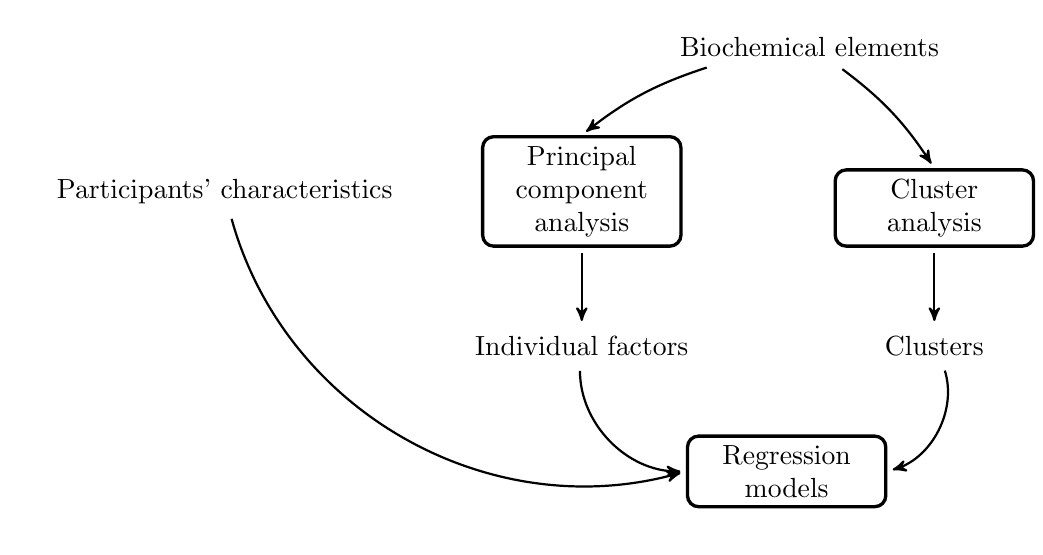
\begin{tikzpicture}[node distance=1cm, auto,]
 \node[punkt](reg){Regression models};
 \node[above=of reg](dummy){};
 \node[left=of dummy](if){Individual factors}
edge[pil,bend right=45](reg.west);
 \node[right=of dummy](c){Clusters}
edge[pil,bend left=45](reg.east);
\node[punkt,above=of if](pca){Principal component analysis}
edge[pil,bend left=0](if.north);
\node[punkt,above=of c](ca){Cluster analysis}
edge[pil,bend left=0](c.north);
\node[left=of pca](cara){Participants' characteristics}
edge[pil,bend right=45](reg.west);
\node[above=of pca](dummy2){};
\node[right=of dummy2](me){Biochemical elements}
edge[pil,bend left =10](ca.north)
edge[pil,bend right=10](pca.north);
\end{tikzpicture}
\captionof{figure}{Global approach in our work.}
  \label{fig:ga}
\begin{flushleft}
{\footnotesize  
It is important to emphasize that principal component analysis and cluster analysis are \emph{exploratory methods} contrary to regression models which predict an outcome. In our work, we separated these two radically different approaches in different chapters.}
\end{flushleft}
\end{figure}

\section{Exploratory methods}

%%%%%%%%%%%%%%%%%%%%%%%%%%%%%%%%%%%%%%%%%%%%%%%%%%%%%%%%
%%%%%%%%%%%%%%%%%%%%%%%%%%%%%%%%%%%%%%%%%%%%%%%%%%%%%%%%

\subsection{First method: PCA}
\emph{Principal component analysis} (PCA) is a statistical tool reducing the dimensions of data. This is particularly interesting when the number of variables $p$ is large in order to summarize the information. Basically, we want to project the $p$-dimensional vectors into a $q$-dimension subspace where $q \ll p$. Our summary will be the projection of the original $p$ vectors on to $q$ directions, the principal components (PCs), which span the subspace. A way of deriving the PCs is to find the projections which maximize the variance. The mathematical demonstration we reported below is taken from the book \emph{Advanced Data Analysis from an Elementary Point of View} by Shalizi \cite{pca_book}.

Let $\mathbf{X}$ be a data of size $n \times p$ where $n$ is the number of individuals and $p$ is the number of variables and let $\mathbf{\tilde{X}_c}$ denote the centered reduced data. Let $\mathbf{x_i}$ denote the $i$-th row of $\mathbf{\tilde{X}_c}$. We are looking for the unit vector $\mathbf{w}$ of size $p \times 1$ such that the variance of the projected individuals on it is maximized, i.e. the PC. 

\newpage

The variance is:

\begin{align*}
\hat{\sigma^2} \big ( \overrightarrow{w}\cdot \overrightarrow{x_i} \big ) &= \frac{1}{n} \sum_{i=1}^n \big ( \overrightarrow{x_i}\cdot \overrightarrow{w} \big )^2 \\
&= \frac{1}{n} \big (\textbf{Xw})^T (\textbf{Xw}) \\
&= \frac{1}{n} \textbf{w}^T \textbf{X}^T \textbf{Xw} \\
&= \textbf{w}^T \frac{\textbf{X}^T \textbf{X}}{n} \textbf{w}. \\
\end{align*}

Thus, we want to maximize $\hat{\sigma^2} (\overrightarrow{w}\cdot \overrightarrow{x_i}) $ with the constraint that $\overrightarrow{w} \cdot \overrightarrow{w} =1$. We will use the Lagrangian function with the Lagrange multiplier $\lambda$:

\begin{align*}
\mathcal{L} (\textbf{w},\lambda) & = \textbf{w}^T \frac{\textbf{X}^T \textbf{X}}{n} \textbf{w} - \lambda (\textbf{w}^T \textbf{w} -1) \\
\frac{\partial \mathcal{L}}{\partial \lambda} & = \textbf{w}^T\textbf{w} -1 \\
\frac{\partial \mathcal{L}}{\partial w} & = 2\frac{\textbf{X}^T \textbf{X}}{n} \textbf{w} - 2 \lambda \textbf{w}. \\
\end{align*} 

\newpage

Setting the derivatives to zero, we get:

\begin{align*}
\textbf{w}^T \textbf{w} & = 1 \\
\frac{\textbf{X}^T \textbf{X}}{n} \textbf{w} & = \lambda \textbf{w}. \\
\end{align*}

The solution is given by diagonalization of matrix $\mathbf{\frac{X^T X}{n}}$ which is in fact the covariance matrix. We obtain $p$ eigenvectors $\mathbf{w}$ that are the principal components (PCs)\footnote{also called \emph{loadings}} and $p$ associated eigenvalues $\lambda$. The maximizing vector will be the one associated with the largest eigenvalue $\lambda$. Eigenvalues are directly proportional to the contribution of their associated PC to the total variance. By nature of diagonalization, the PCs are orthogonal to each other.

All individuals and variables can then be projected on the PCs in order to find some homogeneous patterns of variables or individuals in the data. These projections are called \emph{factors} or \emph{scores}.

Other PCA results are:
\begin{itemize}
\item \emph{Cosine}: the correlation between the variable and the factor \cite{tille_multivariate_nodate},
\item \emph{Squared cosine}: measures the quality of the representation of the variable by a factor \cite{tille_multivariate_nodate}.
\end{itemize}

Following the methodology of Pang et al., we performed a PCA on all urine element excretions \cite{pang_metal_2016}. Before running the PCA, we standardized the variables to unit variance and zero mean.

Using the Elbow method, we selected the first 3 PCs. The Elbow method consists in finding the eigenvalues that are on the left of the line that separates the rapidly decreasing eigenvalues and the approximately equal eigenvalues (Figure \ref{fig:elbow}) \cite{abdi_principal_2010}. Another method for significant PC selection is to select all principal components with eigenvalues greater than 1 \cite{tille_multivariate_nodate}. Using the latter method in this study would mean selecting 7 PCs, which is excessive. As shown by Trevor Hastie et al., we computed the eigenvalues on a normally simulated data $X_{sim}$ of the same dimension as $\tilde{X}_c$, with all $n\cdot p$ cells with unit variance and zero mean \cite{james_introduction_2013}. Values from the simulated data are represented by blue crosses in Figure \ref{fig:elbow}. Only the first 3 eigenvalues are bigger than the simulated ones, which brings us to the same conclusion as for the Elbow method.

\begin{figure}
\centering
\captionsetup{singlelinecheck = false, format= hang, justification=raggedright, font=small, labelsep=space}
\includegraphics[width=0.45\linewidth]{elbow}
\captionof{figure}{Selecting significant principal components.}
  \label{fig:elbow}
\begin{flushleft}
{\footnotesize  Using the Elbow method, we selected the first 3 principal components. The Elbow method consists in finding the eigenvalues that are on the left of the line that separates the rapidly decreasing eigenvalues and the approximately equal eigenvalues (red line). Eigenvalues from normally simulated data are represented by blue crosses. Only the first 3 eigenvalues are bigger than the simulated ones.}
\end{flushleft}
\end{figure}

%%%%%%%%%%%%%%%%%%%%%%%%%%%%%%%%%%%%%%%%%%%%%%%%%%%%%%%%
%%%%%%%%%%%%%%%%%%%%%%%%%%%%%%%%%%%%%%%%%%%%%%%%%%%%%%%%

\subsection{Second method: cluster analysis}
In this section, we will firstly introduce some general considerations on clustering methods and distance metrics. Afterwards, we will describe the three main steps we followed to construct our clusters:
\begin{enumerate}
\item Computing a \emph{distance matrix}: the Manhattan matrix \cite{hennig_handbook_2016},
\item Choosing a clustering algorithm: the PAM algorithm \cite{hennig_handbook_2016},
\item Selecting the number of clusters: the silhouette index \cite{hennig_handbook_2016,kaufman_finding_1990}.
\end{enumerate}

\subsubsection{General considerations on clustering methods}
\emph{Cluster analysis} is a method of finding homogeneous groups in data \cite{kaufman_finding_1990}. These groups are called \emph{clusters}. The number of clusters $K$ is either chosen in function of cluster validation indexes (\emph{parametric clustering}) or itself determined by the clustering method (\emph{nonparametric clustering}) \cite{hennig_handbook_2016}. Clustering methods are unsupervised methods since their aim is not to predict a response variable. After clustering, members assigned to the same cluster are expected to be close to each other in the $p$-dimension space. If the $p$ variables are continuous, this proximity can be defined in terms of Euclidean distance. However other distance metrics exist: the Minkowski-type distance, the Hausdorff distance, the Mahahanobis distance, the Gower dissimilarity, etc \cite{hennig_handbook_2016}. Cluster analysis should not be confused with linear discriminant analysis. Whereas the aim of clustering methods is to establish groups, the aim of linear discriminant analysis is to assign individuals to groups which are already established \cite{hennig_handbook_2016,tille_multivariate_nodate}.

Different types of distances are:
\begin{enumerate}
\item \textbf{Standard Euclidean distance}. If $p$ is the number of variables, the standard Euclidean distance between individuals $x_i$ and $x_j$ and denoted by $d(x_i,x_j)$ is given by:
\begin{equation*}
d(x_i,x_j)=\sqrt{\sum_{l=1}^p (x_{il} - x_{jl} )^2},
\end{equation*}
where $x_{il}$ and $x_{jl}$ are the values taken in variable $l$ by individuals $x_i$ and $x_j$, respectively.
\item \textbf{Manhattan distance}. If $p$ is the number of variables, the Manhattan distance between individuals $x_i$ and $x_j$ and denoted by  $d(x_i,x_j)$ is given by:
\begin{equation*}
d(x_i,x_j)=\sum_{l=1}^p \mid x_{il} - x_{jl} \mid,
\end{equation*}
where $x_{il}$ and $x_{jl}$ are the values taken in variable $l$ by individuals $x_i$ and $x_j$, respectively.

Instead of taking the square of the differences, we are taking the absolute value of the differences. This distance is typically used when adding one unit to $x_{i1}$ and one unit to $x_{i2}$ is the same than adding two units to $x_{i1}$ for any individual $i$ \cite{kaufman_finding_1990}.
\item \textbf{Minkowski distance}. The Euclidean and the Manhattan distances are special cases of the so-called Minkowski distance where $q=2$ for Euclidean distance and $q=1$ for Manhattan distance in the formula below. If $p$ is the number of variables, the Minkowski distance between individuals $x_i$ and $x_j$ and denoted by $d(x_i,x_j)$ is given by:
\begin{equation*}
d(x_i,x_j)= \Big ( \sum_{l=1}^p \mid x_{il} - x_{jl} \mid^q \Big )^{1/q},
\end{equation*}
where $x_{il}$ and $x_{jl}$ are the values taken in variable $l$ by individuals $x_i$ and $x_j$, respectively \cite{hennig_handbook_2016}.
\item \textbf{Gower dissimilarity}. When the Euclidean and the Manhattan distances are distance metrics for continuous variables, the so-called \emph{Gower dissimilarity} allows to aggregate $p$ variables of mixed type. If the data does not contain any missing value the Gower dissimilarity between individuals $x_i$ and $x_j$ and denoted by  $d_G(x_i,x_j)$ is given by:
\begin{equation*}
d_G(x_i,x_j) = \frac{\sum_{l=1}^p w_j \cdot d_l(x_{il},x_{jl})}{\sum_{j=1}^p w_j},
\end{equation*}
where $d_l(x_{il},x_{jl})$ is the Manhattan distance between individuals $x_i$ and $x_j$ for variable $l=1,2\dots p$ \cite{hennig_handbook_2016}. As reported by Hennig et al., Gower recommended to use weights $w_l$ to scale the distances for each variable between 0 and 1 such that $w_j\cdot d_l(x_il,x_jl) \in [0,1]$ for all possible pairs of $x_j$ and $x_j$ individuals. However, Hennig et al. argued to reserve them only for binary and ``very discrete variables'' because otherwise the weights could have an excessive high influence on the cluster borders. Hennig et al. also said that weights may be used in order to give more importance to some variables that are considered as main variables \cite{hennig_handbook_2016}.
\end{enumerate}

\subsubsection{Clustering procedure}

\paragraph{First step: computing the distance matrix.}
The Manhattan distance matrix is computed between all the individuals taking into consideration all standardized urine excretions. The result can then be presented as a $n \times n$ distance matrix. In our case, the distance matrix has dimension $608 \times 608$. The function \texttt{daisy()} from the \texttt{cluster} packcage in \texttt{R} computes the distance matrix. In one-line code we obtained our Manhattan distance matrix:
\begin{verbatim}
mydaisy<-daisy(...,metric = "manhattan")
\end{verbatim}

\paragraph{Second step: choosing a clustering algorithm (PAM).}
The heuristic \emph{partitioning around medoids} (PAM) algorithm belongs to the $k$-medoids clustering methods. The idea behind $K$-medoids is not dissimilar to that of $k$-means. However, whilst we are sampling random points in the $p$-dimension space in $k$-means, we are sampling existing points in $k$-medoids. Compared to $k$-means clustering, this is often a more robust method since it generally does not consider the squared Euclidean distance which is very sensitive to extreme outliers. PAM is an \emph{hard} clustering method. In \emph{hard} clustering, members are assigned to a precise cluster $k$ with null probability of belonging to the $K-1$ remaining clusters. In contrast, in \emph{soft} clustering every member has a degree of membership to each $K$ cluster \cite{hennig_handbook_2016}.

\newpage

The PAM algorithm follows the procedure described in the book \emph{Handbook of Cluster Analysis} by C. Hennig et al. 2016 \cite{hennig_handbook_2016} in five steps:
\begin{displayquote}
\begin{enumerate}
\item Initialize: randomly select (without replacement) $K$ of the $N$ data points as the initial medoids\footnote{However, Kaufman et al. recommend to take non-random data points as the initial medoids \cite{kaufman_finding_1990}.}.
\item Assign each observation to the medoid with which it is closest, where closest is based on a specific distance measure and compute the total cost across all observations, where the cost is the sum of the distance of each observation to its associated medoid.
\item For each medoid $k$, for $k=1$,\dots ,$K$ consider all $N-K$ nonmedoid, $o$. Swap $k$ and $o$ and recompute the total cost.
\item Select the solution with the lowest cost.
\item Repeat steps 2-4 until the set of medoids does not change.
\end{enumerate}
\end{displayquote}

Finding the $K$ medoids is an optimizing problem with a globally optimal solution since we have a finite number of ${N}\choose{K}$ candidate solutions. However, computational cost is often huge in practice. For example, for $N=500$ and $K=5$ which is a realistic example in practice, we would have $2\cdot 10^{11}$ possible sets of medoids and thus $2\cdot 10^{11}$ costs to compute. With the PAM algoritm, only $K \cdot (N-K)$ costs are computed during the first iteration (2475 in our example).

Let us take a simple example to illustrate the PAM algorithm with $n=10$ individuals and 2 variables, $x$ and $y$. Our objective will be to construct two clusters ($K=2$). This data was generated by \texttt{R}:
\begin{verbatim}
set.seed(123)
data<-runif(20)
x<-data[1:10]
y<-data[11:20]
\end{verbatim}

The data is presented in Table \ref{table:dataex}. The corresponding Euclidean distance matrix is shown in Table \ref{table:distmex}. The first iteration of a $k$-medoids algorithm is shown in Figure \ref{fig:pamex2}. In step 1, observations 7 and 9 are randomly chosen as medoids $m_1$ and $m_2$, respectively. In step 2, the sum of the distances is computed in this configuration, assigning the non-medoids to their closest medoid ($\text{cost}_0 = 2.97$). In steps 3 and 4, $m_1$ is swapped with observation 1 as this decreases the sum of the distances by -1.59. Steps 2-4 are repeated until medoid stabilization is achieved. See the \emph{Appendix} for the PAM program used to solve this example.

\begin{table}
\centering
\captionof{table}{Example data for a $k$-medoids algorithm.}
\begin{tabular}{p{2.5cm} p{2cm} p{2cm} }
\toprule
ID & x & y \\
\midrule
\input{dataex.txt}
\bottomrule
\end{tabular}
\label{table:dataex}
\end{table}

\begin{table}
\centering
\captionof{table}{Distance matrix for the example given in Table 4.1.}
\begin{tabular}{ r | rrrrrrrrr}
\toprule
     & 1  &  2  &  3  &  4   & 5  &  6  &  7    &8  &  9 \\
\midrule
2&  0.71      \\                                   
3 & 0.30& 0.44        \\                            
4  &0.71& 0.15& 0.49       \\                        
5 & 1.07 &0.38 &0.78& 0.47    \\                     
6 & 0.25& 0.87& 0.43& 0.90 &1.20       \\              
7 & 0.75& 0.33& 0.45 &0.48& 0.44& 0.81        \\
8 & 1.10 &0.42& 0.80 &0.53& 0.08&1.21 &0.42           \\
9 & 0.68 &0.27& 0.38 &0.41& 0.45&0.76 &0.09 &0.44      \\
10& 0.17& 0.60& 0.28 &0.57& 0.98 &0.41 &0.71 &1.01& 0.63 \\
\bottomrule
\end{tabular}
\label{table:distmex}
\end{table}

\begin{figure}
\captionsetup{singlelinecheck = false, format= hang, justification=raggedright, font=small, labelsep=space}
\includegraphics[width=0.45\linewidth]{pamex_s1} \hfill
\includegraphics[width=0.45\linewidth]{pamex_s2} \\
\includegraphics[width=0.45\linewidth]{pamex_s3} \hfill
\includegraphics[width=0.45\linewidth]{pamex_s4} \\
\captionof{figure}{First iteration of the algorithm for the example given in Table 4.1.}
\label{fig:pamex2}
{\footnotesize In \textbf{step 1}, observations 7 and 9 are randomly chosen as medoids $m_1$ and $m_2$, respectively. In \textbf{step 2}, the sum of the distances is computed in this configuration, assigning the non-medoids to their closest medoid ($\text{cost}_0 = 2.97$). In \textbf{steps 3 and 4}, $m_1$ is swapped with observation 1 as this decreases the sum of the distances by -1.59. Steps 2-4 are repeated until medoid stabilization is achieved.}
\end{figure}

The PAM algorithm was implemented with SKIPOGH data using the \texttt{pam()} function from the \texttt{cluster} package in \texttt{R} \cite{rblog}.

\paragraph{Third step: selecting the number of clusters.}
To select the optimal number of clusters, we computed the \emph{silhouette index}, also called \emph{silhouette width}, for $K=1,2,\dots 10$. The number of clusters $K$ associated with the biggest silhouette index was selected. The silhouette index $SI_K$ is defined as \cite{kaufman_finding_1990}:
\begin{equation*}
SI_K = \frac{1}{n} \sum_{i=1}^n \frac{b(i)-a(i)}{max\{a(i),b(i)\}},
\end{equation*}
where $a(i)$ is the average dissimilarity between object $i$ and all objects in its cluster and $b(i)$ is the minimum average dissimilarity of $i$ to all points in any other cluster not including $i$ \cite{hennig_handbook_2016}. In our work we used the Manhattan dissimilarity. The silhouette index is bounded between minus one and one, i.e. $SI_K \in [-1,1]$.

\newpage

As reported by Struyf et al. \cite{JSSv001i04}, the value $SI_K$ may be interpreted as follows:

\begin{displayquote}
\begin{itemize}
\item $SI_K \approx 1 \Rightarrow$ object $i$ is well classified (in $A$),
\item $SI_K \approx 0 \Rightarrow$ object $i$ lies intermediate between two clusters ($A$ and $B$),
\item $SI_K \approx -1 \Rightarrow$ object $i$ is badly classified (closer to $B$ than to $A$).
\end{itemize}
\end{displayquote}

Thus, the higher the index is, the more distinguishable the clusters are. Conceptually, the silhouette index measures the distance between the clusters whilst taking into account out each cluster is (see examples in Figure \ref{fig:silex}). Not only can the silhouette index be used as a tool to chose the optimal number of clusters, but also to measure the quality of the clustering result and thereby is an index for cluster validation.

\begin{figure}
\captionsetup{singlelinecheck = false, format= hang, justification=raggedright, font=small, labelsep=space}
\includegraphics[width=0.45\linewidth]{siex1} \hfill
\includegraphics[width=0.45\linewidth]{siex2} \\
\includegraphics[width=0.45\linewidth]{siex3} \hfill
\includegraphics[width=0.45\linewidth]{siex4} \\
\captionof{figure}{Examples of silhouette index.}
\label{fig:silex}
{\footnotesize These plots show 4 situations concerning 2 clusters (white and black). They illustrate that the silhouette index takes into consideration both the size of the clusters and the distance between each other. Plot a) where the clusters are far and small has the highest silhouette index ($SI_K=0.772$). Plot b) where the clusters are far and big and plot c) where the clusters are close and small have the same silhouette index ($SI_K=0.543$). Plot d) where the clusters are close and big has the lowest silhouette index ($SI_K=0.190$).}
\end{figure}

%%%%%%%%%%%%%%%%%%%%%%%%%%%%%%%%%%%%%%%%%%%%%%%%%%%%%%%%
%%%%%%%%%%%%%%%%%%%%%%%%%%%%%%%%%%%%%%%%%%%%%%%%%%%%%%%%

\section{Assessing for cluster stability}
If we state that our data is a random sample from a finite population, we can consider clustering as a random process. In this scope, clusters are random. However, we would like to construct $K$ clusters from our data that are the more stable as possible. In order to assess for cluster stability, we will summary two methods:

\begin{enumerate}
\item \textbf{The Rand index} \cite{rand_objective_1971}. The \emph{Rand index} is a measure of cluster stability. Firstly, we divide the data of dimension $n \times p$ into three parts: two training sets $S$ and $T$ and one testing set $E$. Then, we perform a clustering on $S$ giving $\mathcal{C}_S$ and on $T$ giving $\mathcal{C}_T$, independently. The purpose is to use points of $E$ to see if there is a difference in cluster attribution if we are using the medoids of $\mathcal{C}_S$ or the medoids of $\mathcal{C}_T$. The rand index is given by:
\begin{equation*}
\mathcal{R}(\mathcal{C}_S,\mathcal{C}_T)=\frac{N_{11}+N_{00}}{n(n-1)/2},
\end{equation*}

where $N_{11}$ is the number of point pairs of $E$ that are in the same cluster with both $\mathcal{C}_S$ and $\mathcal{C}_T$ and where $N_{00}$ is the number of point pairs of $E$ in different clusters with both $\mathcal{C}_S$ and $\mathcal{C}_T$ \cite{hennig_handbook_2016}.

Since Rand index is random from the sampling step, a bootstrap version combining a kind of Rand index and bootstrap techniques was described by Dolnicar and Leisch in 2010 \cite{dolnicar_evaluation_2010}.

\item \textbf{Bootstrapping average cluster stability} \cite{dolnicar_evaluation_2010}. The technique computes several replicates of Rand indices with the notable difference that $S_i$ and $T_i$ are both bootstrapped samples of size $n$ from the original data that replace $S$ and $T$ in the classical Rand index. The formula for the replicates is:

\begin{equation*}
\mathcal{R}_i(\mathcal{C}_{S_i},\mathcal{C}_{T_i})=\frac{N_{{11}_i}+N_{{00}_i}}{n(n-1)/2},
\end{equation*}
where $N_{{11}_i}$ is the number of point pairs of $E$ that are in the same cluster under both $\mathcal{C}_{S_i}$ and $\mathcal{C}_{T_i}$ and where $N_{{00}_i}$ is the number of point pairs of $E$ in different clusters under both $\mathcal{C}_{S_i}$ and $\mathcal{C}_{T_i}$ \cite{dolnicar_evaluation_2010}. The mean and the standard deviations of bootstrapped replicates are estimates of expectation and standard error of Rand index, respectively.
\end{enumerate}

%%%%%%%%%%%%%%%%%%%%%%%%%%%%%%%%%%%%%%%%%%%%%%%%%%%%%%%%
%%%%%%%%%%%%%%%%%%%%%%%%%%%%%%%%%%%%%%%%%%%%%%%%%%%%%%%%

\section{Checking for assumptions}
Statistical test results are not presented if assumptions are violated. For every performed two-sided two-sample Student’s test, normality in the two groups was assessed using normal Q-Q plots. Moreover, equal variance assumption was adopted if the $p$-value in the Levene's test was larger than $5\%$.



%%%%%%%%%%%%%%%%%%%%%%%%%%%%%%%%%%%%%%%%%%%%%%%%%
% Results
%%%%%%%%%%%%%%%%%%%%%%%%%%%%%%%%%%%%%%%%%%%%%%%%%

\chapter{Results}

%%%%%%%%%%%%%%%%%%%%%%%%%%%%%%%%%%%%%%%%%%%%%%%%%
% Results
%%%%%%%%%%%%%%%%%%%%%%%%%%%%%%%%%%%%%%%%%%%%%%%%%

In the first section, we describe the data. In the second section, exploratory analyses are presented. Subsequent sections study the link between the biochemical elements and hypertension.

\section{Global data description}
For each continuous variable, the mean, the standard deviation (SD), the median, the interquartile range (IQR), the skewness and the kurtosis were given (see Table \ref{table:des_cont}). The mean age was 48.1 years (SD=17.8). All metal-mixtures without exception had a positive skewness and a positive kurtosis. This is often seen in variables measuring concentrations since negative concentrations do not exist and extreme values are easy to reach with intoxication and/or impaired physiology. Aluminum, platine, cobalt and thallium kurtosis had extremely high kurtosis, respectively 461, 561, 324 and 576. This is partially due to extreme outliers. Indeed, if we removed the highest thallium value (36763.83 ng), the skewness passed from 23.8 to 1.5, the kurtosis passed from 576 to 6 and the boxplot of the variable completely changed (see Figure \ref{fig:Tl_eo}). Sample kurtosis is extremely sensitive to extreme outliers since its formula is spreading the difference between the mean and a value with power 4:

\begin{equation*}
kurtosis=\frac{n\cdot(n+1)\cdot(n-1)}{(n-2)\cdot(n-3)} \frac{\sum_{i=1}^n (x_i- \bar{x})^4}{(\sum_{i=1}^n (x_i- \bar{x})^2)^2}.
\end{equation*}

However, it is possible for a participant to have this thallium value since 36700 ng = 36 mg and severe poisoning begins with values higher than 1000 mg. Thus, we decided to keep this high value. Similarly, other metal-mixture were showing highest values that were often under their lethal dose. Consequently, we decided to keep these high values since we cannot exclude mild intoxication cases.

\begin{table}
\centering
\captionof{table}{Description of continuous variables ($n=608$, $35$ variables).}
\begin{adjustbox}{max width = 14cm}
\begin{tabular}{lrrrrrr}
\toprule
Variable & Mean & SD & Median & IQR & Skew. & Kurt. \\
\midrule
\input{des_cont_var.txt}
\bottomrule
\end{tabular}
\end{adjustbox}
\label{table:des_cont}
\end{table}

\begin{figure}
\captionsetup{singlelinecheck = false, format= hang, justification=raggedright, font=small, labelsep=space}
\includegraphics[width=0.45\linewidth]{outlier1} \hfill
\includegraphics[width=0.45\linewidth]{outlier2} 
\captionof{figure}{Effect of removing the biggest thallium concentration.}
\label{fig:Tl_eo}
{\footnotesize \textbf{Left}: distribution of thallium concentrations in ng from original data. \textbf{Right}: distribution of thallium concentrations in ng after removing the highest value. As we can see, the thallium boxplot completely changed after removing the highest value.}
\end{figure}

Discrete variables are reported in Table \ref{table:des_cat} ($n=608$, $4$ variables) where they are simply expressed as counts and proportions. There were 290 men and 318 women. 4.6\% of the participants had diabetes. Hypertension concerned 23.3\% of the participants. This is slightly lower than the worldwide prevalence estimated to $26.4\%$ ($95\% \text{ CI } 26.0-26.8\%$) \cite{kearney_global_2005}.

\begin{table}
\centering
\captionof{table}{Description of discrete variables ($n=608$, $4$ variables).}
\begin{adjustbox}{max width = 14cm}
\begin{tabular}{llrr}
\toprule
Variable & Reference Category & Reference cases (\%) & Non ref. cases (\%) \\
\midrule
Sex	& \emph{male} &  290 (47.7\%) &  318 (52.3\%) \\
Diabetes & \emph{has diabetes} & 28 \hspace{1pt} (4.6\%) & 580 (95.4\%) \\
Anti-hypertensive drugs & \emph{taking drugs} & 99 (16.3\%) & 509 (83.7\%) \\
Medical hypertension & \emph{has hypertension} & 142 (23.3\%) & 466 (76.7\%) \\
\bottomrule
\end{tabular}
\end{adjustbox}
\label{table:des_cat}
\end{table}

\section{Exploratory analysis}

In this section, correlation matrix, PCA and cluster analysis are presented.

\subsection{Correlation matrix}
Correlation matrix was computed using Pearson's method. All metal-mixtures and non-metals are only positively correlated between each other. Moreover, the correlation between vanadium and chrome (0.87, $p$-value $<0.05$ in the correlation test) and the correlation between phosphates and urea (0.78, $p$-value $<0.05$ in the correlation test) are the strongest ones (see Figure \ref{fig:correlation_metals}). If correlation between vanadium and chrome is difficult to interpret, the correlation between phosphates and urea can be explained by two reasons. Firstly, it can result from the increased level of these biochemical elements often seen in \emph{chronic kidney disease} which concerns at least 6\% of the population (US survey) \cite{kasper_harrisons_2015}. Secondly, it can be a consequence of a diet rich in meat where both urea and phosphates intakes increase.

\begin{figure}
\centering
\captionsetup{singlelinecheck = false, format= hang, justification=raggedright, font=small, labelsep=space}
\includegraphics[width=1\linewidth]{CorrM}
\captionof{figure}{Correlation plot representing correlations between 24-hour urine excretions.}
  \label{fig:correlation_metals}
\begin{flushleft}
{\footnotesize This plot graphically represents correlations between metal-mixtures and non-metals with rounds (Pearson's correlations) with the color intensity directly proportional to the correlation value. Non significant ($p$-value $>0.05$) correlations are expressed as a crossed round. This plot underlines the fact that all metal-mixtures and non-metals correlate only positively between each other. Moreover, the strongest correlations are between vanadium and chrome (0.87) and between phosphates and urea (0.78).}
\end{flushleft}
\end{figure}

\subsection{PCA}

\subsubsection{PCA results}
Plots showing the variables factor map and individuals factor map from PCA are shown in Figure \ref{fig:pca_var} and Figure \ref{fig:pca_ind}, respectively. Factor loadings are presented in Table \ref{table:floadings}. Three PCs explained 46.04\% of the total variance. Loadings with absolute value greater than 0.40 were considered as important and reported in bold in Table \ref{table:floadings}. The first PC (explaining 31.71\% of the variance) represents the global exposure to metal-mixtures and non-metals since they are all positively correlated with the PC. The second PC (explaining 8.57\% of the variance) is almost more interesting than the first PC since it is only correlated with non-metals (sodium, calcium, phosphates, urea and magnesium). Therefore, it can be assumed that this PC underlies the fact that the sources and/or the metabolic pathways are not the same between metal-mixtures and non-metals the data. This difference between metal-mixtures and non-metals can also be seen in Figure \ref{fig:pca_var} where metal-mixtures (in maroon) are approximately orthogonal to non-metals (in orange), and therefore linearly independent in the two-dimentional space of the PCA. The third PC (only explaining 5.76\% of the variance) is correlated with silver and bismuth.

A supplementary plot displays the 5 essential metal-mixtures (manganese, cobalt, copper, zinc and molybdenum) in black and the 17 remaining toxic metal-mixtures in gray on the variables factor map (Figure \ref{fig:pca_toxic}). Interestingly, this indicates that all the essential metal-mixtures are present in the positive values of the second axis.

\begin{figure}
\centering
\captionsetup{singlelinecheck = false, format= hang, justification=raggedright, font=small, labelsep=space}
\includegraphics[width=0.75\linewidth]{pca_var}
\captionof{figure}{PCA of variables.}
  \label{fig:pca_var}
\begin{flushleft}
{\footnotesize Metal-mixtures and non-metals are represented in maroon and orange respectively.}
\end{flushleft}
\end{figure}

\begin{figure}
\centering
\captionsetup{singlelinecheck = false, format= hang, justification=raggedright, font=small, labelsep=space}
\includegraphics[width=0.75\linewidth]{pca_ind}
\captionof{figure}{PCA of individuals.}
  \label{fig:pca_ind}
\begin{flushleft}
{\footnotesize Red dots represent individuals with hypertension (hta). Black dots represent individual with no hypertension (no hta).}
\end{flushleft}
\end{figure}

\begin{table}
\centering
\captionof{table}{Factor loadings in PCA.}
\begin{tabular}{lrrrrrr}
\toprule
Variable & PC 1 & PC 2 & PC 3 \\
\midrule
lithium, ng&\textbf{0.521}&0.126&-0.023\\
beryllium, ng&\textbf{0.570}&0.171&0.100\\
aluminum, ng&\textbf{0.527}&0.396&0.204\\
vanadium, ng&\textbf{0.836}&-0.075&-0.039\\
chrome, ng&\textbf{0.799}&-0.054&0.010\\
manganese, ng&\textbf{0.485}&0.295&0.217\\
cobalt, ng&\textbf{0.497}&0.222&-0.324\\
nickel, ng&\textbf{0.706}&0.200&-0.279\\
copper, ng&\textbf{0.588}&0.158&-0.357\\
zinc, ng&\textbf{0.548}&0.045&-0.322\\
arsenic, ng&0.374&0.173&0.169\\
molybdenum, ng&\textbf{0.578}&0.048&-0.387\\
palladium, ng&\textbf{0.645}&-0.091&-0.166\\
silver, ng&\textbf{0.407}&0.264&\textbf{0.517}\\
cadmium, ng&\textbf{0.531}&0.199&-0.100\\
tin, ng&\textbf{0.411}&0.204&-0.071\\
antimony, ng&\textbf{0.491}&0.145&-0.145\\
platinum, ng&\textbf{0.605}&-0.032&-0.115\\
mercury, ng&\textbf{0.585}&0.112&0.250\\
thallium, ng&\textbf{0.727}&0.041&-0.109\\
lead, ng&\textbf{0.522}&0.340&0.202\\
bismuth, ng&0.373&0.317&\textbf{0.563}\\
sodium, mmol&\textbf{0.575}&\textbf{-0.460}&0.173\\
potassium, mmol&\textbf{0.540}&-0.328&0.298\\
calcium, mmol&0.354&\textbf{-0.508}&0.078\\
phosphate, mmol&\textbf{0.552}&\textbf{-0.599}&0.049\\
urea, mmol&\textbf{0.586}&\textbf{-0.621}&0.115\\
magnesium, mmol&\textbf{0.500}&\textbf{-0.471}&0.054\\
\midrule
Eigenvalue & 8.878 & 2.401 & 1.613 \\
Total variance (\%) & 31.71 & 8.57 &  5.76 \\
Cumulative (\%) & 31.71 &  40.28 & 46.04 \\
\bottomrule
\end{tabular}
\label{table:floadings} \\
{\footnotesize Factor loadings are given in bold if $>0.40$.}
\end{table}

\begin{figure}
\centering
\captionsetup{singlelinecheck = false, format= hang, justification=raggedright, font=small, labelsep=space}
\includegraphics[width=0.75\linewidth]{pca_toxic}
\captionof{figure}{PCA of variables with metal-mixture type.}
  \label{fig:pca_toxic}
\begin{flushleft}
{\footnotesize \textbf{In black}: the 5 essential metal-mixtures (manganese, cobalt, copper, zinc and molybdenum). \textbf{In gray}: the 17 remaining toxic metal-mixtures and the non-metals. All the essential metal-mixtures without exception are in the upper right quadrant.}
\end{flushleft}
\end{figure}

Note that we cannot see heterogenous distribution of the individuals with hypertension and those without hypertension in the individuals factor map in Figure \ref{fig:pca_ind}.

\subsection{Cluster analysis}

\paragraph{Clustering results.}
The Manhattan distance matrix from SKIPOGH was computed as explained in Chapter \ref{ch:Methods}. It is of a considerable size ($608 \times 608$). Consequently, we only presented it in a graphical way in Figure \ref{fig:distancematrix} where each point is a pixel in an image of size $608 \times 608$ picture. Each pixel in this image represents the distance between one individual and another. Pixels are sorted by participant ID. The brighter the pixel is, the greater the distance is. Naturally, we cannot distinguish patterns in the matrix before the clustering procedure. 

\begin{figure}
\centering
\captionsetup{singlelinecheck = false, format= hang, justification=raggedright, font=small, labelsep=space}
\includegraphics[width=0.45\linewidth]{distancematrix}
\captionof{figure}{Manhattan distance matrix ($608 \times 608$).}
  \label{fig:distancematrix}
\begin{flushleft}
{\footnotesize Each pixel in this image represents the distance between one individual and another. Pixels are sorted by participant ID. The brighter the pixel is, the greater the distance is. Naturally, we cannot distinguish patterns in the matrix before the clustering procedure. }
\end{flushleft}
\end{figure}

From the calculation of silhouette width, the optimal number of clusters was set as 2 (Figure \ref{fig:silhouette}). Consequently, PAM algorithm was runned with $K=2$. The cost after the build phase was $22.0$ and the cost after the swap phase was $21.6$. Silouhette width was 0.1767. The clusters are detailed in Table \ref{table:cdes}. The first and the second clusters had 249 and 359 individuals, respectively. The distance matrix before and after clustering are compared in Figure \ref{fig:distancematrix2}.

\begin{figure}
\centering
\captionsetup{singlelinecheck = false, format= hang, justification=raggedright, font=small, labelsep=space}
\includegraphics[width=0.45\linewidth]{silhouette}
\captionof{figure}{Graphic of silhouette width.}
  \label{fig:silhouette}
\begin{flushleft}
{\footnotesize The graph shows that the optimal number of clusters is 2 as this yiels the greatest silhouette width.}
\end{flushleft}
\end{figure}

\begin{table}
\centering
\captionof{table}{Obtained clusters description ($K=2$).}
\begin{tabular}{rrrrr}
\toprule
Size  & maximum diss.  & average diss.  & diameter & separation \\
\midrule
249 & 48.04068 &21.15747 &67.54185 & 11.88677 \\
359& 38.60081 &21.89540& 60.45442 & 11.88677\\
\bottomrule
\end{tabular}
\label{table:cdes}
\end{table}

\begin{figure}
\centering
\captionsetup{singlelinecheck = false, format= hang, justification=raggedright, font=small, labelsep=space}
\includegraphics[width=0.45\linewidth]{dma} \hfill
\includegraphics[width=0.45\linewidth]{dmb} 
\captionof{figure}{Distance matrix before and after clustering.}
\label{fig:distancematrix2}
\begin{flushleft}
{\footnotesize a) Distance matrix sorted by participant ID, b) Distance matrix ordered by cluster attribution: the 249 observations on the left belong to cluster 1 and the 359 observations on the right belong to cluster 2. We can see slightly lower distances between individuals belonging to the same cluster.}
\end{flushleft}
\end{figure}

\paragraph{Clustered individuals in the space of the PCA.}
The two clusters display different biochemical patterns for first two PCs of the PCA as edvidenced by their boxplots and associated two-sided two-sample Student’s tests (see Figure \ref{fig:ttestc1c2}). Interpretation of the first PC of the PCA shows that the second cluster has a higher global exposure to metal-mixtures and non-metals. As for the second PC, the second cluster also has higher concentrations of non-metals.

\begin{figure}
\centering
\captionsetup{singlelinecheck = false, format= hang, justification=raggedright, font=small, labelsep=space}
\includegraphics[width=0.45\linewidth]{ttestc1} \hfill
\includegraphics[width=0.45\linewidth]{ttestc2} 
\captionof{figure}{Individual factors (PCA) by cluster attribution.}
\label{fig:ttestc1c2}
\begin{flushleft}
{\footnotesize \textbf{Left}: the second cluster has a higher global exposure to metal-mixtures and non-metals ($p$-value of the Student's test $<0.05$). \textbf{Right}: the second cluster has higher concentrations of non-metals ($p$-value of the Student's test $<0.05$).}
\end{flushleft}
\end{figure}

\paragraph{Assessing for cluster stability.}
Since we performed PAM algorithm from the Manhattan distance matrix, we wanted to compare cluster stability with PAM algorithm performed from a Euclidean distance matrix. We studied the replicates of the Rand index as explained in chapter \ref{ch:Methods}. We fixed at $B=1000$ the number of replications. Results are shown in Table \ref{table:bootr} and Figure \ref{fig:boot}. According to the Mann-Whitney test, PAM algorithm from the Manhattan distance matrix provides higher replicates than PAM algorithm from the Euclidean distance matrix, at level $\alpha=5\%$. Consequently, we kept the Manhattan metric.

\begin{table}
\centering
\captionof{table}{Bootstrapped replicates of the Rand index.}
\begin{tabular}{rrr}
\toprule
Metric  & Mean  & SD \\
\midrule
Euclidean & 0.084 &  0.149 \\
Manhattan & 0.103 & 0.155 \\
\bottomrule
\end{tabular}
\label{table:bootr}
\end{table}

\begin{figure}
\centering
\captionsetup{singlelinecheck = false, format= hang, justification=raggedright, font=small, labelsep=space}
\includegraphics[width=0.45\linewidth]{stabmetric}
\captionof{figure}{Boxplot of bootstrapped replicates of the Rand index, $B=1000$.}
  \label{fig:boot}
\begin{flushleft}
{\footnotesize Boxplots describing the bootstrapped replicates of the Rand index in function of the metric chosen. According to the Mann-Whitney test, PAM algorithm from the Manhattan distance matrix provides higher replicates than PAM algorithm from the Euclidean distance matrix, at level $\alpha=5\%$. Consequently, we kept the Manhattan metric.}
\end{flushleft}
\end{figure}

\section{Link with the outcome}
In this section, previously found individual scores from PCA and clusters from cluster analysis are linked with hypertension as depicted in Figure \ref{fig:ga}. The first part will use simple association analyses and subsequent parts will use regression methods.

\subsection{Simple association analyses}
In Figure \ref{fig:PCscores}, individual factors by hypertension status are summarized in boxplots for dimension 1 and dimension 2, respectively. Two-sided two-sample Student’s tests were performed on the two first dimensions to compare the \emph{hypertension} and \emph{no hypertension} groups. The results of the two-sided two-sample Student’s tests are presented in Table \ref{table:ttestout}. According to the $p$-values from two-sided two-sample Student’s tests, mean in dimension 1 is lower in hypertensive individuals than in non-hypertensive individuals at level $\alpha=5\%$ but difference of means between hypertensive and non-hypertensive groups in dimension 2 is not statistically significant at level $\alpha=5\%$.

\begin{figure}
\centering
\captionsetup{singlelinecheck = false, format= hang, justification=raggedright, font=small, labelsep=space}
\includegraphics[width=0.45\linewidth]{PC1scores} \hfill
\includegraphics[width=0.45\linewidth]{PC2scores} 
\captionof{figure}{Individual PC 1 and PC 2 scores by hypertension status.}
\label{fig:PCscores}
\begin{flushleft}
{\footnotesize hta: hypertension. No hta: no hypertension.}
\end{flushleft}
\end{figure}

\begin{table}
\centering
\captionof{table}{Means of the individual factors by hypertension status.}
\begin{tabular}{lrrr}
\toprule
Group & Dim 1 & Dim 2 & $p$-value \\
\midrule
hta & -0.6466 & 0.0712 & 0.003 \\
no hta & 0.1970 &  -0.0216 & 0.532 \\
\bottomrule
\end{tabular}
\label{table:ttestout}
\begin{flushleft}
{\footnotesize According to the $p$-values from the two-sided two-sample Student’s tests, mean in dimension 1 is lower in \emph{hta} individuals than in \emph{no hta} individuals at level $\alpha=5\%$ but difference of means between \emph{hta} and \emph{no hta} groups in dimension 2 is not statistically significant at level $\alpha=5\%$. \\
hta: hypertension. No hta: no hypertension.}
\end{flushleft}
\end{table}

Continuous outcomes are SBP and DBP. A Pearson's correlation matrix was computed between SBP, DBP and individual factors. The correlation matrix is shown in Table \ref{table:cortoprint}. The magnitude of the correlations between SBP, DBP and the individual factors is small, even if they are significant at level $\alpha=5\%$.

\begin{table}
\centering
\captionof{table}{Correlation matrix between the 1st PC, the 2nd PC, SBP and DBP.}
\begin{tabular}{l|rrrr}
\toprule
Variable & 1st PC & 2nd PC & SBP & DBP \\
\midrule
1st PC & 1.00 &  & &   \\
2nd PC & 0.00 & 1.00 &  & \\
SBP  &\textbf{-0.12} &-0.02&  1.00 &  \\
DBP  & 0.03& \textbf{-0.09} & \textbf{0.67} & 1.00 \\
\bottomrule
\end{tabular}
\label{table:cortoprint} \\
{\footnotesize Significant correlations at level $\alpha=5\%$ are given in bold.}
\end{table}

Note that these significant results are only associations between variables and hence do not considerate confounding effects that may also influence blood pressure. In contrast, later used multiple regressions allow this adjustment.
 
\subsection{Individual factors as independent variables}
We performed three models incorporating individual factors as independent variables.

Models $M1$ and $M2$ are multiple linear regression models predicting SBP and DBP, respectively. First, two scores in $COMP1$ and $COMP2$ from PCA were used as independent variables in these two models. Both $M1$ and $M2$ are adjusted for participants' characteristics. Covariates come from the non-standardized log-transformed data as explained in Chapter \ref{ch:Data} and models are also adjusted for hypertension treatment $d_{hta}$ since hypertension treatment lowers both SBP and DBP. Thereby, hypertension treatment has a confounding effect. 

\subsubsection{Model M1}
The equation of $M1$ modeling SBP is given by:
\begin{align*}
SBP_i &=  \beta_0 + \beta_1 \cdot COMP1_i+ \beta_2 \cdot COMP2_i + \beta_3 \cdot age_i + \beta_4 \cdot sex01_i  \\
& +\beta_5 \cdot diabetes_i +\beta_6 \cdot tg_i +\beta_7 \cdot cho_i +\beta_8 \cdot glu_i +\beta_9 \cdot ins2s_i \\
&+ \beta_{10} \cdot d_{hta,i}+ \epsilon_i.
\end{align*}

The multiple R-squared of this model is 0.3748 (adjusted R-squared = 0.3644). The estimates of $\beta$ coefficients are presented in Table \ref{table:betasm1}.

\begin{table}
\centering
\captionof{table}{Estimated regression coefficients from model $M1$.}
\begin{tabular}{lrrrrl}
\toprule
Variable & Estimate & Std. error & $t$-value & $P(|T|>|t|)$ &\\
\midrule
(Intercept)& 78.849436 &  5.631900& 14.001 & $<$ 2e-16&*  \\
comp1    &   -0.225694  & 0.200761&  -1.124 &0.261383   &  \\
comp2  &     -0.064776  & 0.395809 & -0.164& 0.870058   &  \\
age      &    0.385600  & 0.040689 &  9.477 & $<$ 2e-16&* \\
sex01M    &   4.534503   &1.342142 &  3.379 &0.000776&*  \\
diabetes   &  2.371990  & 3.379602 &  0.702 &0.483043   &  \\
tg     &      1.786916 &  0.946166  & 1.889 &0.059432  &\\
cho       &   0.515524  & 0.657140 &  0.784 &0.433060  &  \\ 
glu         & 2.486982 &  1.046957  & 2.375& 0.017843&*  \\
ins2s    &   0.008919  & 0.089712 &  0.099& 0.920842 &  \\  
d\_htaYes    & 7.934874  & 1.753170 &  4.526& 7.26e-06&*  \\
\bottomrule
\end{tabular}
\label{table:betasm1} \\
{\footnotesize An asterisk (*) indicates significant coefficients at level $\alpha=5\%$.}
\end{table}

For abbreviations please refer to \emph{Appendix}. The Fisher test for model $M1$ is significant at level $\alpha=0.05$ with an $F$-statistic = 35.79. As seen in Table \ref{table:betasm1}, the Student's test is significant for variables $age$, $sex01M$, $glu$ and $d_{hta}$ at level $\alpha=0.05$. Thus, unsurprisingly age and male sex predict a higher SBP prediction as reported in the medical literature. Glucose is also predicting a higher SBP. This can be explained by the fact that both diabetes and hypertension belong to the Metabolic Syndrome as defined in Chapter \ref{ch:Context}. Less intuitively, having antihypertensive treatment predicts a higher SBP. We can however state that people taking medications are less healthy and consequently more likely to develop hypertension.

\subsubsection{Model M2}
The equation of $M2$ modeling DBP is given by:
\begin{align*}
DBP_i &=  \beta_0 + \beta_1 \cdot COMP1_i+ \beta_2 \cdot COMP2_i + \beta_3 \cdot age_i + \beta_4 \cdot sex01_i  \\
& +\beta_5 \cdot diabetes_i +\beta_6 \cdot tg_i +\beta_7 \cdot cho_i +\beta_8 \cdot glu_i +\beta_9 \cdot ins2s_i \\
&+ \beta_{10} \cdot d_{hta,i}+ \epsilon_i.
\end{align*}

The multiple R-squared of model $M2$ is 0.1726 (adjusted R-squared 0.1587). Consequently, variability of DBP is less explained by our covariates than variability of SBP in model $M1$. The estimates of $\beta$ coefficients are presented in Table \ref{table:betasm2}.

\begin{table}
\centering
\captionof{table}{Estimated regression coefficients from model $M2$.}
\begin{tabular}{lrrrrl}
\toprule
Variable & Estimate & Std. error & $t$-value & $P(|T|>|t|)$& \\
\midrule
(Intercept)& 50.60413  &  3.61834 & 13.985 & $<$ 2e-16&* \\
comp1      &  0.12540 &   0.12898  & 0.972& 0.331344 & \\  
comp2    &   -0.30491   & 0.25430&  -1.199 &0.230996  & \\  
age        &  0.09867 &   0.02614 & 3.775& 0.000176&* \\
sex01M    &  3.21195  &  0.86229 &  3.725 &0.000214&*  \\
diabetes  &  -6.98053  & 2.17130 & -3.215& 0.001375&*  \\ 
tg       &    1.06510  &  0.60789 &  1.752& 0.080263 &\\ 
cho     &     0.97064 &   0.42219 &  2.299 &0.021848&*  \\
glu       &   2.25712  &  0.67264   &3.356& 0.000842&* \\
ins2s       & 0.01834  &  0.05764&   0.318 &0.750441  & \\  
d\_htaYes    & 1.64266  &  1.12636 &  1.458& 0.145264  & \\  
\bottomrule
\end{tabular}
\label{table:betasm2} \\
{\footnotesize An asterisk (*) indicates significant coefficients at level $\alpha=5\%$.}
\end{table}

The Fisher test for model $M2$ is significant at level $\alpha=0.05$ with an $F$-statistic=12.45. Again age and male sex contribute to a higher blood pressure prediction. Here, cholesterol has a significant positive coefficient at level $\alpha=0.05$. This can be explained by the fact that high cholesterol levels belong to the Metabolic Syndrome. Suprinsingly, the results indicate that diabetes predicts lower DBP. There are two possible explanations:
\begin{itemize}
\item Non-significant covariates can make noise,
\item Glucose interacts with diabetes. This could be physiologically possible since diabetics with higher glucose have more severe diabetes.
\end{itemize}

Consequently we computed a reduced version of model $M2$ that we called model $M2r$ with only significant covariates of model $M2$ at level $\alpha=0.05$ and an interaction between glucose and diabetes. However we kept $COMP1$ and $COMP2$ in this new model since they are the covariates of interest. The equation of model $M2r$ is given by:
\begin{align*}
DBP_i &=  \beta_0 + \beta_1 \cdot COMP1_i+ \beta_2 \cdot COMP2_i + \beta_3 \cdot age_i + \beta_4 \cdot sex01_i  \\
& + \beta_5 \cdot cho_i + \beta_6 \cdot glu_i + \beta_7 \cdot diabetes_i + \beta_8 \cdot glu_i \times diabetes_i \\
& +\epsilon_i.
\end{align*}

The multiple R-squared of model $M2r$ is similar to multiple R-squared of model $M2$ with 0.1790 (adjusted R-squared 0.1680). The Fisher test is significant at level $\alpha=0.05$ with an $F$-statistic=16.33. The estimates of $\beta$ coefficients are presented in Table \ref{table:betasm2r}.

\begin{table}
\centering
\captionof{table}{Estimated regression coefficients from model $M2r$.}
\begin{tabular}{lrrrrl}
\toprule
Variable & Estimate & Std. error & $t$-value & $P(|T|>|t|)$ &\\
\midrule
(Intercept)&  42.76614 &   3.96295 & 10.791 & $<$ 2e-16&*  \\
comp1   &      0.10582   & 0.12789   &0.827 &0.408329  &  \\ 
comp2   &     -0.35875&    0.25167  &-1.425& 0.154535   &  \\
age        &   0.09504 &   0.02457  & 3.868 &0.000122&*  \\
sex01M    &    3.35733 &   0.84546  & 3.971& 8.03e-05&*  \\
cho       &    1.14073  &  0.39600  & 2.881& 0.004111&*  \\
glu        &   3.89406    &0.76967 &  5.059& 5.60e-07&*  \\
diabetes    & 25.57865 &   9.53225 &  2.683& 0.007490&* \\ 
glu:diabetes &-4.80809  &  1.39674 & -3.442 &0.000617&*  \\
\bottomrule
\end{tabular}
\label{table:betasm2r} \\
{\footnotesize An asterisk (*) indicates significant coefficients at level $\alpha=5\%$.}
\end{table}

It is now less surprising to see that both glucose and diabetes predict higher DBP in this model (positive coefficients). Interestingly, there is a significant negative interaction between glucose and diabetes which signifies that diabetic participants have a smaller increase in DBP by glucose increments. This can be explained by the arterial stiffness in people suffering from diabetes. Arteries in diabetic people are less likely to be elastic and consequently, their volume cannot adapt to pressure variations, leading to a greater difference between DBP and SBP readings. The result is a higher SBP but a lower DBP as measured by \emph{pulse pressure} ($PP$):
\begin{equation*}
PP=SBP-DBP.
\end{equation*}

Indeed, pulse pressure ($PP$) is higher in diabetics and has even been showed to increase hospitalization events in diabetics \cite{yu_association_2015}. The negative regression coefficient for this interaction in model $M2r$ could be a result explained by pulse pressure. This effect could be investigated with models predicting $PP$ instead of $SBP$ and $DBP$ in diabetics. However, this is beyond the scope of this study.

Neither the $M1$ nor the $M2$ models show significant coefficients for $COMP1$ and $COMP2$. Classical risk factors for hypertension such as age, sex and diabetes are better predictors.

\subsubsection{Model M3}
We tried a third model ($M3$) modeling the binary variable (logistic regression). The equation of model $M3$ is given by:
\begin{align*}
log \Bigg (\frac{hta_i}{1-hta_i} \Bigg ) &=  \beta_0 + \beta_1 \cdot COMP1_i+ \beta_2 \cdot COMP2_i + \beta_3 \cdot age_i + \beta_4 \cdot sex01_i  \\
& +\beta_5 \cdot diabetes_i +\beta_6 \cdot tg_i +\beta_7 \cdot cho_i +\beta_8 \cdot glu_i +\beta_9 \cdot ins2s_i,
\end{align*}

where $hta$ is the binary variable defining hypertension status (1: hypertension, 0: no hypertension). Note that model $M3$ is not adjusted for hypertension treatment since $hta$ is defined by $d_{hta}$ ($y$ is assumed to be random).

In model $M3$, null deviance is 660.94 on 607 degrees of freedom and residual deviance is 462.69 on 598 degrees of freedom. The likelihood ratio test of model $M3$ using the Chi-squared test has the $p$-value $<0.05$, i.e. we reject the null hypothesis $H_0$ that the model with only the intercept is appropriate at level $\alpha=0.05$. The estimates of $\beta$ coefficients are presented in Table \ref{table:betasm3}.

\begin{table}
\centering
\captionof{table}{Estimated Regression coefficients from model $M3$.}
\begin{tabular}{lrrrrl}
\toprule
Variable & Estimate & Std. error & $z$-value & $P(|Z|>|z|)$ &\\
\midrule
(Intercept)& -6.630614 &  1.965623 & -3.373 &0.000743& * \\
comp1      &  0.026360 &  0.044178  & 0.597& 0.550718   &  \\
comp2    &    0.033556&   0.085314   &0.393 &0.694077   &  \\
age     &     0.083365  & 0.009397 &  8.871  & $<$ 2e-16 &* \\
sex01M &      0.171037  & 0.279701&   0.611 &0.540869    & \\
diabetes  &   0.638388 &  0.558014 &  1.144& 0.252609  &   \\
tg         &  0.689512  & 0.272210  & 2.533 &0.011309& *  \\ 
cho     &    -0.161488   &0.132422  &-1.219 &0.222658    & \\
glu      &    0.781633 &  1.170823  & 0.668& 0.504393    & \\
ins2s     &   0.219532&  0.149054&   1.473& 0.140796& \\
\bottomrule
\end{tabular}
\label{table:betasm3} \\
{\footnotesize An asterisk (*) indicates significant coefficients at level $\alpha=5\%$.}
\end{table}

In this logistic model, age and triglycerides have positive estimated coefficients. All other coefficients are non-significant, especially $COMP1$ and $COMP2$.

\subsection{Cluster ID as an independent variable}
We performed multiple regressions with being in cluster 2 (\emph{cluster2} below) as the independent binary variable.

Models $M4$ and $M5$ are linear regression models predicting SBP and DBP, respectively, and are adjusted for participants' characteristics. Covariates come from the non-standardized log-transformed data as explained in Chapter \ref{ch:Data} and models are also adjusted for hypertension treatment $d_{hta}$. Model $M6$ is a logistic model predicting the binary variable (1: hypertension, 0: no hypertension).

\subsubsection{Model M4}
The equation of model $M4$ modeling SBP is given by:
\begin{align*}
SBP_i &= \beta_0 + \beta_1 \cdot cluster2 + \beta_2 \cdot age_i + \beta_3 \cdot sex01_i  \\
& +\beta_4 \cdot diabetes_i +\beta_5 \cdot tg_i +\beta_6 \cdot cho_i +\beta_7 \cdot glu_i +\beta_8 \cdot ins2s_i \\
& + \beta_9 \cdot d_{hta,i}+ \epsilon_i.
\end{align*}

The multiple R-squared of this model is 0.3898 (adjusted R-squared = 0.3806). The estimates of $\beta$ coefficients are presented in Table \ref{table:betasm4}.

\begin{table}
\centering
\captionof{table}{Estimated regression coefficients from model $M4$.}
\begin{tabular}{lrrrrl}
\toprule
Variable & Estimate & Std. error & $t$-value & $P(|T|>|t|)$ &\\
\midrule
(Intercept)& 74.14797 &   9.51703&   7.791& 2.95e-14& * \\
cluster2   & -0.70356 &   1.26813  &-0.555 & 0.57924    & \\
age      &    0.38766   & 0.04002  & 9.688 & $<$ 2e-16 & * \\
sex01M   &    4.18226  &  1.30988  & 3.193 & 0.00148& * \\
diabetes    & 1.88478  &  3.14829&   0.599 & 0.54962  & \\  
tg        &   2.75999  &  1.26919   &2.175 & 0.03005 &*  \\
cho    &      0.15756  &  0.66226 &  0.238 & 0.81203  & \\
glu  &       12.08047 &   5.87012 &  2.058 & 0.04003 &*  \\
ins2s     &   1.64967 &   0.69877 &  2.361 & 0.01855& * \\  
d\_htaYes   &  7.45125  &  1.72414   &4.322 &1.81e-05 &* \\
\bottomrule
\end{tabular}
\label{table:betasm4} \\
{\footnotesize An asterisk (*) indicates significant coefficients at level $\alpha=5\%$.}
\end{table}

The Fisher test for model $M4$ is significant at level $\alpha=0.05$ with an $F$-statistic = 42.44. As seen in Table \ref{table:betasm4}, the Student's test is significantly positive for 6 variables that were already discussed in previous models. However, the estimated coefficient for $cluster2$ is not significant at level $\alpha=0.05$, thereby suggesting no effect of being in cluster 2 on SBP.

\subsubsection{Model M5}
The equation of $M5$ modeling DBP is given by:
\begin{align*}
DBP_i &= \beta_0 + \beta_1 \cdot cluster2 + \beta_2 \cdot age_i + \beta_3 \cdot sex01_i  \\
& +\beta_4 \cdot diabetes_i +\beta_5 \cdot tg_i +\beta_6 \cdot cho_i +\beta_7 \cdot glu_i +\beta_8 \cdot ins2s_i \\
&+ \beta_9 \cdot d_{hta,i}+ \epsilon_i.
\end{align*}

The multiple R-squared of this model is 0.1878 (adjusted R-squared = 0.1756). The estimates of $\beta$ coefficients are presented in Table \ref{table:betasm5}.

\begin{table}
\centering
\captionof{table}{Estimated regression coefficients from model $M5$.}
\begin{tabular}{lrrrrl}
\toprule
Variable & Estimate & Std. error & $t$-value & $P(|T|>|t|)$ &\\
\midrule
(Intercept) &42.27783&    6.13165 &  6.895 &1.37e-11& *\\
cluster2    & 1.32460   & 0.81703&   1.621& 0.105494   & \\
age       &   0.09046  & 0.02578  & 3.509& 0.000484 &* \\
sex01M    &   2.97388 &   0.84393 &  3.524 &0.000458 &* \\
diabetes &   -6.91662   & 2.02838 & -3.410 &0.000694 &* \\
tg       &    1.57705  &  0.81772&   1.929& 0.054254 & \\
cho      &   0.80436 &   0.42668&   1.885& 0.059891 & \\
glu      &   13.02165  &  3.78201  & 3.443& 0.000615& * \\
ins2s     &   0.69425   & 0.45020 &  1.542& 0.123583  &  \\
d\_htaYes   &  1.39602   & 1.11083  & 1.257& 0.209340   &  \\
\bottomrule
\end{tabular}
\label{table:betasm5} \\
{\footnotesize An asterisk (*) indicates significant coefficients at level $\alpha=5\%$.}
\end{table}

The Fisher test for model $M5$ is significant at level $\alpha=0.05$ with an $F$-statistic = 15.36. As seen in Table \ref{table:betasm5}, the Student's test is significantly positive for 4 variables but the estimated coefficient for $cluster2$ is not significant at level $\alpha=0.05$, thereby suggesting no effect of being in cluster 2 on DBP.

\subsubsection{Model M6}
We tried a sixth model ($M6$) modeling the binary variable (logistic regression). The equation of model $M6$ is given by:
\begin{align*}
log \Bigg (\frac{hta_i}{1-hta_i} \Bigg ) &= \beta_0 + \beta_1 \cdot cluster2 + \beta_2 \cdot age_i + \beta_3 \cdot sex01_i  \\
& +\beta_4 \cdot diabetes_i +\beta_5 \cdot tg_i +\beta_6 \cdot cho_i +\beta_7 \cdot glu_i +\beta_8 \cdot ins2s_i,
\end{align*}

where $hta$ is the binary variable defining hypertension status (1: hypertension, 0: no hypertension). In model $M6$, null deviance is 660.94 on 607 degrees of freedom and residual deviance is 463.07 on 599 degrees of freedom. Likelihood ratio test of model $M6$ using the Chi-squared test has the $p$-value $<0.05$. The estimated of $\beta$ coefficients are presented in Table \ref{table:betasm6}.

\begin{table}
\centering
\captionof{table}{Estimated Regression coefficients from model $M6$.}
\begin{tabular}{lrrrrl}
\toprule
Variable & Estimate & Std. error & $z$-value & $P(|Z|>|z|)$ &\\
\midrule
(Intercept)& -6.807494 &  1.969900 & -3.456 &0.000549 &* \\
cluster2 &    0.122215 &  0.275414 &  0.444& 0.657224    & \\
age       &   0.082373  & 0.009025 & 9.127  & $<$ 2e-16 &* \\
sex01M    &   0.121431 &  0.278675 &  0.436& 0.663023  &   \\
diabetes   &  0.623978 &  0.556553  & 1.121 &0.262225  &   \\
tg          & 0.683021&   0.271457  & 2.516& 0.011865 &*   \\
cho       &-0.165296&  0.132238 & -1.250& 0.211304  &   \\
glu        &  0.938256   &1.158391 &  0.810& 0.417961  &   \\
ins2s       & 0.196607 &  0.146601&  1.341& 0.179889 & \\
\bottomrule
\end{tabular}
\label{table:betasm6} \\
{\footnotesize An asterisk (*) indicates significant coefficients at level $\alpha=5\%$.}
\end{table}

The Wald test is significat for 2 variables but the estimated coefficient for $cluster2$ is not significant at level $\alpha=0.05$, thereby suggesting no effect of being in cluster 2 on the binary outcome.

\section{Other regression models}
We were also interested in comparing previously found models ($M1$, $M2$, $M3$, $M4$, $M5$ and $M6$) with other multiple regression models. We created the models $MA$ modelling SBP, $MB$ modelling DBP and $MC$ modelling the binary variable $hta$. These models were selected using backward elimination steps with the goal of minimizing the Akaike information criterion (AIC). Full model contained all variables in \emph{urine} data except SBP, DBP and the binary outcome $hta$.

\subsubsection{Model MA}
$MA$ models SBP. After the minimizing process, AIC passed from 4921 ($df=38$) to 4888 ($df=16$). The multiple R-squared of this model is 0.4264 (adjusted R-squared = 0.4129). The estimates of $\beta$ coefficients are presented in Table \ref{table:betasma}. 14 variables were selected using backward elimination steps minimizing the AIC. Over these variables, 7 are metal-mixtures: vanadium, nickel, zinc, molybdenum, cadmium, platinum and bismuth. 

\begin{table}
\centering
\captionof{table}{Estimated regression coefficients from model $MA$.}
\begin{tabular}{lrrrrl}
\toprule
Variable & Estimate & Std. error & $t$-value & $P(|T|>|t|)$& \\
\midrule
(Intercept)&  75.73552&   15.83771  & 4.782& 2.19e-06&*  \\
age       &    0.39657  &  0.04375  & 9.065 & $<$ 2e-16&* \\
sex01M     &   3.58861  &  1.23375  & 2.909  &0.00377&*  \\
d\_htaYes    &  6.81367   & 1.67018&   4.080& 5.13e-05&* \\
tg         &   2.96728 &   1.16086&   2.556 & 0.01083&*    \\
glu       &    8.82544   & 5.36468  & 1.645&  0.10048  &   \\
ins2s       &  1.51136 &   0.69479 & 2.175&  0.03000&*  \\
V\_h24\_excr &   6.37188    &1.54939 &  4.113& 4.47e-05&* \\
Ni\_h24\_excr & -1.90769   &1.04873 & -1.819&  0.06941 & \\  
Zn\_h24\_excr&   2.00974  &  1.02100 &  1.968&  0.04949&*  \\
Mo\_h24\_excr  &-2.54884&    1.01466 & -2.512 & 0.01227&* \\  
Cd\_h24\_excr & -1.85876   & 1.15642 & -1.607 & 0.10851 &\\    
Pt\_h24\_excr & -2.48081  & 0.90931  &-2.728&  0.00656 &* \\
Bi\_h24\_excr&   0.73415  &  0.48182&   1.524&  0.12812  & \\  
umg\_u24\_mmol& -0.62031 &   0.38567  &-1.608 & 0.10828 & \\   
\bottomrule
\end{tabular}
\label{table:betasma} \\
{\footnotesize An asterisk (*) indicates significant coefficients at level $\alpha=5\%$.}
\end{table}

For abbreviations please refer to \emph{Appendix}. The Fisher test for model $MA$ is significant at level $\alpha=0.05$ with an $F$-statistic = 31.49. As evidenced in Table \ref{table:betasma}, vanadium and zinc have significant positive coefficients at level $\alpha=0.05$ and molybdenum and platinum have significant negative coefficients at level $\alpha=0.05$.

\subsubsection{Model MB}
$MB$ models DBP. After the minimizing process, AIC passed from 4418 ($df=38$) to 4379 ($df=13$). The Multiple R-squared of this model is 0.1948 (adjusted R-squared = 0.1799). This supports the earlier finding which indicates that it is more difficult to model SBP than DBP. The estimates of $\beta$ coefficients are presented in Table \ref{table:betasmb}. 11 variables were selected using backward elimination steps minimizing the AIC. Over these variables, only 3 are metal-mixtures: nickel, antimony and bismuth. However, none of them are significant at level $\alpha=0.05$.

\begin{table}
\centering
\captionof{table}{Estimated regression coefficients from model $MB$.}
\begin{tabular}{lrrrrl}
\toprule
Variable & Estimate & Std. error & $t$-value & $P(|T|>|t|)$ &\\
\midrule
(Intercept)&   47.560254  & 8.113291  & 5.862 &7.58e-09&* \\
age         &   0.110698&   0.024187 &  4.577& 5.75e-06&* \\
sex01M    & 2.923871&   0.840597  & 3.478 &0.000541&* \\
diabetes   &   -6.314285  & 2.023708&  -3.120 &0.001895&* \\ 
tg         &    1.920339  & 0.814985 & 2.356 &0.018781&*   \\
cho         &   0.693786 &  0.423921 &  1.637& 0.102243  & \\ 
glu         &  10.152343  & 3.913886  & 2.594 &0.009722&* \\
ins2s       &   0.901545 &  0.469622  & 1.920& 0.055369 & \\
Ni\_h24\_excr  &-0.980218 &  0.625635 & -1.567& 0.117702&\\    
Sb\_h24\_excr    &0.716485 &  0.424483 &  1.688 &0.091954&\\ 
Bi\_h24\_excr   & 0.488656  & 0.315137  & 1.551& 0.121526 & \\  
uure\_u24\_mmol & 0.006593 &  0.003662 &  1.800& 0.072326 &\\
\bottomrule
\end{tabular}
\label{table:betasmb} \\
{\footnotesize An asterisk (*) indicates significant coefficients at level $\alpha=5\%$.}
\end{table}

The Fisher test for model $MB$ is significant at level $\alpha=0.05$ with an $F$-statistic = 13.11.

\subsubsection{Model MC}
$MC$ models the binary outcome. After the minimizing process, AIC passed from 511 ($df=36$) to 472 ($df=11$). Null deviance is 660.94 on 607 degrees of freedom and residual deviance is 449.87 on 597 degrees of freedom. The likelihood ratio test of model $MC$ using the Chi-squared test has the $p$-value $<0.05$, i.e. we reject the null hypothesis $H_0$ that the model with only the intercept is appropriate at level $\alpha=0.05$. The estimates of $\beta$ coefficients are presented in Table \ref{table:betasmc}.

\begin{table}
\centering
\captionof{table}{Estimated regression coefficients from model $MC$.}
\begin{tabular}{lrrrrl}
\toprule
Variable & Estimate & Std. error & $z$-value & $P(|Z|>|z|)$ &\\
\midrule
(Intercept) &  -11.414821  & 2.878483 & -3.966 & 7.32e-05 &*\\
age      &      0.091363  & 0.009714 &  9.405  & $<$ 2e-16 &*\\
diabetes     &  0.774399  & 0.520395 &  1.488& 0.136725    & \\
tg          &   0.868417  & 0.251146  & 3.458 &0.000545 &*\\
cho       &    -0.192934&   0.133184 & -1.449 &0.147441    & \\
Zn\_h24\_excr   &0.473567 &  0.209705  & 2.258 &0.023930 &*  \\
Ag\_h24\_excr &  -0.192466  &0.109058 & -1.765& 0.077598 & \\
Pt\_h24\_excr   &-0.374779 & 0.205700 & -1.822 &0.068460 &  \\
Tl\_h24\_excr &   0.422767  & 0.268637 &  1.574 &0.115546   &  \\
uk\_u24\_mmol   & 0.011549 &  0.006583&   1.754 &0.079376&  \\
umg\_u24\_mmol  &-0.161155 &  0.094318&  -1.709& 0.087518&  \\
\bottomrule
\end{tabular}
\label{table:betasmc} \\
{\footnotesize An asterisk (*) indicates significant coefficients at level $\alpha=5\%$.}
\end{table}

In model $MC$, age, triglycerides and zinc are increasing the predicted probablity to have hypertension according to their significant estimated coefficients at level $\alpha=5\%$.

\subsubsection{Discussion on multiple regressions}
Models $MA$, $MB$ and $MC$ are better models than the previous models in term of R-squared for linear regressions and likelihood ratio tests for logistic regressions.

We found several significant coefficients for metal-mixtures at level $\alpha=5\%$ but none for sodium (una\_u24\_mmol) that is a component of salt which is a classical risk factor for hypertension. This highlights the fact that metal-mixtures are potential risk factors for hypertension. In model $MA$, vanadium and zinc predicted a higher SBP. Both vanadium and zinc are essential metal-mixtures. Moreover, the predicted probability to have hypertension is higher if zinc concentrations increase according to our logistic model ($MC$).  Recently, a Chinese study has shown that participants in the highest quartiles of vanadium and zinc (and some other metal-mixtures) had higher odd ratios for hypertension compared with those in the lowest quartiles \cite{wu_environmental_2018}. Although normal levels of essential-mixtures are important to maintain a normal blood pressure, the authors caution that excessive accumulation of them can lead to hypertension.





%%%%%%%%%%%%%%%%%%%%%%%%%%%%%%%%%%%%%%%%%%%%%%%%%
% Conclusion
%%%%%%%%%%%%%%%%%%%%%%%%%%%%%%%%%%%%%%%%%%%%%%%%%

\chapter{Discussion}

In the SKIPOGH data, 23.3\% of participants had hypertension. This is slightly lower than the worldwide prevalence estimated to $26.4\%$. Exploration of variable distributions showed very skewed distributions with extreme outliers. However, outliers were kept in the exploratory analysis since all were nevertheless realistic concentrations. Interestingly, principal component analysis (PCA) could help to distinguish between metal-mixtures and non-metals.  Thus, despite competition that often occurs between biochemical elements in physiological processes --- notably between elements sharing the same valence --- metal-mixtures and non-metals seem to be uncorrelated. Moreover, essential metal-mixtures were all isolated in the upper right quadrant, again suggesting different sources in dietary intakes or different physiological processes compared to other biochemical elements. However, multiple regression incorporating scores of principal components and adjusted for participants characteristics failed to predict hypertension. Then, two clusters were generated from the $k$-medoids algorithm. They displayed different biochemical patterns. However, silhouette width was small and clusters could not predict hypertension in multiple regressions adjusted for participants characteristics.

In supplementary analyses, we performed other regression models using observed covariates with backward elimination of variables minimizing the Akaike information criterion (AIC). These models performed better than those incorporating PCA and cluster information. Moreover, vanadium and zinc predicted higher SBP, which is consistent with the literature. Moreover, the predicted probability to develop hypertension was higher with increments of zinc concentrations in a logistic regression. This underlines the fact that essential metal-mixtures can lead to hypertension when they are in excessive quantities. However, significant estimated coefficients were not found for mercury and cadmium which are toxic metal-mixtures with cardiovascular effects \cite{cosselman_environmental_2015}.

There are several reasons for finding no significant estimated coefficient for biochemical patterns in the first analyses. Firstly, it is highly likely that main metal-mixtures and non-metals simply contribute little to hypertension compared to classical risk factors for hypertension such as age, male sex and diabetes. Secondly, significant effects can be hidden by non-significant effects in PCA and cluster analysis methods that incorporate all the variables. Restricted choice of variables from medical expertise, adapted regression methods such as minimizing AIC or Lasso and Ridge regressions can deal situations with variables that participate not to the total variance. Moreover, SBP and DBP --- that are not independent between each other --- could be studied together instead of separately in more complex models such as neural networks allowing multiple outputs. Thirdly, longitudinal studies may be more sensitive to detect an association between metal-mixtures and hypertension.

\newpage

In conclusion, if heterogeneous biochemical patterns could be distinguished in the SKIPOGH data, they could predict neither systolic, diastolic blood pressure nor hypertension cases using multiple regressions. Restricted variable selection for multiple regression models gave better models.

%%%%%%%%%%%%%%%%%%%%%%%%%%%%%%%%%%%%%%%%%%%%%%%%%
% Bibliography
%%%%%%%%%%%%%%%%%%%%%%%%%%%%%%%%%%%%%%%%%%%%%%%%%

\bibliography{biblio}
\bibliographystyle{acm}

%%%%%%%%%%%%%%%%%%%%%%%%%%%%%%%%%%%%%%%%%%%%%%%%%
% Appendix
%%%%%%%%%%%%%%%%%%%%%%%%%%%%%%%%%%%%%%%%%%%%%%%%%
\appendix
\appendixpage
\addappheadtotoc

\chapter*{Abbreviations}

\begin{verbatim}
cpnbr: participant number
age: age, years
sex01: sex (1=male)
diabetes: diabetes (1=yes)
d_hta: anti-hypertensive drugs, (1=yes)
tg: triglycerides, mmol/l
cho: cholesterol, mmol/l
glu: blood glucose, mmol/l
ins2s: blood insulin, microIU/ml
Li_h24_excr: lithium, ng
Be_h24_excr: beryllium, ng
Al_h24_excr: aluminum, ng
V_h24_excr: vanadium, ng
Cr_h24_excr: chrome, ng
Mn_h24_excr: manganese, ng
Co_h24_excr: cobalt, ng
Ni_h24_excr: nickel, ng
Cu_h24_excr: copper, ng
Zn_h24_excr: zinc, ng
As_h24_excr: arsenic, ng
Mo_h24_excr: molybdenum, ng
Pd_h24_excr: palladium, ng
Ag_h24_excr: silver, ng
Cd_h24_excr: cadmium, ng
Sn_h24_excr: tin, ng
Sb_h24_excr: antimony, ng
Pt_h24_excr: platinum, ng
Hg_h24_excr: mercury, ng
Tl_h24_excr: thallium, ng
Pb_h24_excr: lead, ng
Bi_h24_excr: bismuth, ng
una_u24_mmol: sodium, mmol
uk_u24_mmol: potassium, mmol
uca_u24_mmol: calcium, mmol
upo4_u24_mmol: phosphate, mmol
uure_u24_mmol: urea, mmol
umg_u24_mmol: magnesium, mmol
sbp_mean: systolic blood pressure, mmHg
dbp_mean: diastolic blood pressure, mmHg
hta: medical hypertension (1=yes)
\end{verbatim}


\chapter*{\texttt{R}-code: PAM program}

\begin{lstlisting}[language=R]
# PAM PROGRAM IN R

# I) Enter the inital cluster configuration
set.seed(123)
data<-runif(20)
x<-data[1:10]
y<-data[11:20]
X<-round(cbind(x,y),2)
X<-cbind(X,c(0,0,0,0,0,0,1,0,1,0))
# We added a third column to specify by "1"
# which observations are initial medoids.
colnames(X)[3]<-"m"
X # X is the initial cluster configuration

# II) create a cost function in function of the
#     current cluster configuration X
cost_fun<-function(X){
  N<-nrow(X)
  K<-sum(X[,3])
  mi<-which(X[,3]==1)
  oi<-which(X[,3]==0)
  costs<-rep(NA,time=N)
  D<-as.matrix(dist(X[,-3],method="euclidean",upper = T,diag=T))
  for(i in 1:N){
    costs[i]<-min(D[i,mi])
  }
  result<-sum(costs)
  return(result)
}

# III)  using cost function, return the next cluster
#       configuration in functon of current configuration
one_it_PAM<-function(X){
  N<-nrow(X)
  K<-sum(X[,3])
  mi<-which(X[,3]==1)
  oi<-which(X[,3]==0)
  ci<-cost_fun(X)
  cost<-rep(NA,time=K*(N-K))
  C<-cbind(expand.grid(mi,oi),cost)
  nswap<-nrow(C)
  for(i in 1:nswap){
    X_swap<-X
    X_swap[C[i,2],3]<-1
    X_swap[C[i,1],3]<-0
    C[i,3]<-cost_fun(X_swap)
  }
  best_swap<-which.min(C[,3])
  X_best<-X
  X_best[C[best_swap,2],3]<-1
  X_best[C[best_swap,1],3]<-0
  if(cost_fun(X_best)<cost_fun(X)) return(X_best)
    else return(X)
}

#############################################
#############################################
#############################################

# Example
X
X2<-one_it_PAM(X)
X2
X3<-one_it_PAM(X2)
X3
X4<-one_it_PAM(X3)
X4 # stabilisation after 2 iterations
\end{lstlisting}

\chapter*{\texttt{R}-code: whole code}

\begin{lstlisting}[language=R]
#################################################
# MASTER THESIS DENIS DERIAZ 2018               #
#                                               #
# APPLICATION ON BIOCHEMICAL CLUSTER DETECTION  #
# PROFESSOR: ALINA MATEI                        #
#################################################

#Working directory
setwd("C:/Users/erabl/Documents/01_Statistiques_UNINE/Master_thesis/urine_analysis20181005")

#Packages used
library(psych) # for LaTeX tables
library(ggplot2) # for correlation matrix
library(ggcorrplot) # for correlation matrix
library(FactoMineR) # for PCA
library(cluster) # for gower similarity and pam
library(flexclust) #randIndex() function
library(car) #levene test

#######################################################################
#######################################################################
###################################################### DATA PREPARATION

#Opening row data: data_urine.txt
XU<-read.table("C:/Users/erabl/Documents/01_Statistiques_UNINE/Master_thesis/data/20181008_SKIPOGH/data_urine1.txt")
#data from "Master_thesis/script00000000.R"

#Missing values
nrow(XU) #1254 obs
missing_count<-XU[1,]
for(i in 1:ncol(missing_count)) missing_count[i]<-length(which(is.na(XU[,i])==T))
t(missing_count)
XUnona<-na.omit(XU)
nrow(XU)     # 1254
nrow(XUnona) # 609

#Histograms of continuous distributions
var_cont<-c(2,6:39)
for(k in var_cont){
  hist(XUnona[,k],main=colnames(XUnona)[k])
}

#Removing max insulin obs
max(XUnona[,9])
which(XUnona[,9]==max(XUnona[,9])) #obs 218
XUnona<-XUnona[-218,]
dim(XUnona)

#We log-transform graphically positive skewed distr
colnames(XUnona) #10:31
XUnonal<-XUnona
for(i in c(10:31)){
  XUnonal[,i]<-log(XUnona[,i])
}

#Checking again for continuous distributions
var_cont<-c(2,6:39)
for(k in var_cont){
  hist(XUnonal[,k],main=colnames(XUnonal)[k])
}

#Standardizing: mean0 sd1
XUnonalstd<-XUnonal[c(10:37)]
for(i in 1:ncol(XUnonalstd)){
  XUnonalstd[,i]<-(XUnonalstd[,i]-mean(XUnonalstd[,i]))/sd(XUnonalstd[,i])
}
XUnonalstd<-cbind(XUnonalstd,XUnona[,40])
dim(XUnonalstd)

#######################################################################
#######################################################################
############################################## VARIABLE CHARACTERISTICS
var_cont<-c(2,6:39)  # label for continuous var
var_cat<-c(3,4,5,40) # label for categorical var

prettynames<-c("participant's number","age, years",
               "sex (1=male)", "diabetes (1=yes)",
               "anti-hypertensive drugs, (1=yes)",
               "triglycerides, mmol/l","cholesterol, mmol/l",
               "blood glucose, mmol/l","blood insulin, microIU/ml",
               "lithium, ng", "beryllium, ng", "aluminum, ng",
               "vanadium, ng", "chrome, ng", "manganese, ng",
               "cobalt, ng", "nickel, ng","copper, ng",
               "zinc, ng","arsenic, ng","molybdenum, ng",
               "palladium, ng","silver, ng","cadmium, ng",
               "tin, ng", "antimony, ng", "platinum, ng",
               "mercury, ng", "thallium, ng", "lead, ng", "bismuth, ng",
               "sodium, mmol", "potassium, mmol", "calcium, mmol",
               "phosphate, mmol", "urea, mmol","magnesium, mmol",
               "systolic blood pressure, mmHg",
               "diastolic blood pressure, mmHg",
               "medical hypertension (1=yes)")

#Description table for continuous var
colnames(XUnona)<-prettynames
des_var_cont<-round(describe(XUnona[var_cont],IQR=T),1)[,-c(1,2,6,7,8,9,10,13)]
des_var_cont<-des_var_cont[c(1,2,3,6,4,5)]
#write.table(des_var_cont,"C:/Users/erabl/Documents/01_Statistiques_UNINE/Master_thesis/thesis/des_cont_var.txt",eol="\\\\\n",quote=F,sep="&",
#            row.names = T,col.names = F)

# Illustration kurtosis
#attach(XUnona)
#png("C:/Users/erabl/Documents/01_Statistiques_UNINE/Master_thesis/thesis/figures/outlier1.png",width = 404, height=404)
#par(mfrow=c(1,1))
#boxplot(`thallium, ng`,main="thallium with eo, ng")
#dev.off()
#png("C:/Users/erabl/Documents/01_Statistiques_UNINE/Master_thesis/thesis/figures/outlier2.png",width = 404, height=404)
#par(mfrow=c(1,1))
#boxplot(`thallium, ng`[-520],main="thallium without eo, ng")
#dev.off()

#Description table for categorical var
for(m in var_cat){
  print(colnames(XUnona)[m])
  print(table(XUnona[,m]))
  print(table(XUnona[,m])/608)
}

# Reasons of hypertension
c_d=0
c_sbp=0
c_dbp=0
for(i in which(XUnona[,40]=="hta")){
  if(XUnona[i,5]=="Yes") c_d=c_d+1
  if(XUnona[i,38]>140) c_sbp=c_sbp+1
  if(XUnona[i,39]>90) c_dbp=c_dbp+1
}
list(nobs_drugs=c_d,nobs_sbp=c_sbp,nobs_dbp=c_dbp)

#######################################################################
#######################################################################
#################################################### CORRELATION MATRIX
colnames(XUnonal)<-prettynames
CM<-cor(XUnonal[,10:37])
pmatCM<-cor_pmat(XUnonal[,10:37])
ggcorrplot(CM,method=c("circle"),colors=c("purple","white","red"),
           p.mat=pmatCM,hc.order = T, type = "lo")
# width 1000 for output

#######################################################################
#######################################################################
################################################################### PCA

#pca objects
pca_ind<-PCA(XUnonalstd,quali.sup = 29)
par(mfrow=c(1,1),cex=0.4)
pca_var<-PCA(XUnonalstd[,-29])
pca_var$eig

#Plot pca var
#png("C:/Users/erabl/Documents/01_Statistiques_UNINE/Master_thesis/thesis/figures/pca_var.png",width = 790,height = 790)
par(mfrow=c(1,1),cex=1.6)
plot(pca_var,col.var = c(rep("maroon",time=22),rep("orange",time=6)),choix = "var",cex=0.9)
#dev.off()

#Plot pca ind
#png("C:/Users/erabl/Documents/01_Statistiques_UNINE/Master_thesis/thesis/figures/pca_ind.png",width = 790,height = 790)
par(mfrow=c(1,1),cex=1.6)
plot(pca_ind,habillage = 29,choix = "ind",col.hab = c("red","black"),
     label = "none",cex=1.4)
#dev.off()

#Plot tox
esslab<-c(0,0,0,0,0,1,1,0,1,1,0,1,rep(0,time=16))
labtox<-rep("gray",time=28)
for(i in 1:28){
  if(esslab[i]==1) labtox[i]<-"black"
}
#png("C:/Users/erabl/Documents/01_Statistiques_UNINE/Master_thesis/thesis/figures/pca_toxic.png",width = 790,height = 790)
#par(mfrow=c(1,1),cex=1.6)
plot(pca_var,col.var = labtox,choix = "var",cex=0.9)
#dev.off()

#comp
comp1<-pca_ind$ind$coord[,1]
comp2<-pca_ind$ind$coord[,2]

#boxplots comp 1 and 2
#png("C:/Users/erabl/Documents/01_Statistiques_UNINE/Master_thesis/thesis/figures/PC1scores.png",width = 404,height = 404)
par(mfrow=c(1,1))
boxplot(comp1~XUnona[,40],main="PC 1 (global exposure)")
#dev.off()
#png("C:/Users/erabl/Documents/01_Statistiques_UNINE/Master_thesis/thesis/figures/PC2scores.png",width = 404,height = 404)
par(mfrow=c(1,1))
boxplot(comp2~XUnona[,40],main="PC 2 (Na-Ca-Po4-urea-Mg)")
#dev.off()
t.test(comp1~XUnona[,40],var.equal=T)
t.test(comp2~XUnona[,40],var.equal=T)

#######################################################################
#######################################################################
############################################################ Clustering

#SPECIFIC DATA PREPARATION FOR CLUSTERING PROCESS

colnames(XUnonal) # current data

boxplot(log(XUnonal[,9])) # insuline needs to be log transformed
boxplot(XUnonal[,6])
boxplot(log(XUnonal[,6])) # tri needs to be log transformed
boxplot(XUnonal[,8])
boxplot(log(XUnonal[,8])) # glu needs to be log transformed

#We log-transform graphically positive skewed distr
colnames(XUnona) #6,8,9,10:31
XUnonal<-XUnona
for(i in c(6,8,9,10:31)){
  XUnonal[,i]<-log(XUnona[,i])
}

#Preparing XUnonal for daisy function
XUnonalG<-XUnonal
for(i in var_cont){
  XUnonalG[,i]<-as.numeric(XUnonal[,i])
}
for(i in var_cat){
  XUnonalG[,i]<-as.factor(XUnonal[,i])
}
colnames(XUnonalG)
var_cont
for(i in var_cont){
  XUnonalG[,i]<-(XUnonalG[,i]-mean(XUnonalG[,i]))/sd(XUnonalG[,i])
}

# CLUSTERING PROCESS

# I) Distance matrix
mydaisy<-daisy(XUnonalG[,10:37],metric = "manhattan")
range(as.matrix(mydaisy))
# mydaisytoplot needs to be between 0 and 1 (0: black, 1: white)
mydaisytoplot<-as.matrix(mydaisy)*0.999999/99.05336
range(mydaisytoplot)
#png("C:/Users/erabl/Documents/01_Statistiques_UNINE/Master_thesis/thesis2/figures/distancematrix.png")
image(1:608,1:608,mydaisytoplot,
      xlab = " ",ylab = " ",main="Distance matrix")
#dev.off()

# II and III) number of clusters
# Calculate silhouette width for many k using PAM
sil_width <- c(NA)
for(i in 2:10){
  pam_fit <- pam(mydaisy,
                 diss = T,
                 k = i)
  sil_width[i] <- pam_fit$silinfo$avg.width
}

#Plot of sihouette width
#png("C:/Users/erabl/Documents/01_Statistiques_UNINE/Master_thesis/thesis2/figures/silhouette.png")
par(mfrow=c(1,1))
plot(1:10, sil_width,
     xlab = "Number of clusters",
     ylab = "Silhouette Width",xlim=c(1,10),xaxt='n')
axis(side = 1, at=2:10)
lines(1:10, sil_width)
abline(v=2,lty=2,col="red")
abline(h=sil_width[2],lty=2,col="red")
#dev.off()
#k=3 shows tho greater silhouette width

#Distance matrix befor and after clustering
mycluster<-pam(mydaisy,diss = TRUE,k = 2)
cluster<-as.factor(mycluster$clustering)
c1<-which(cluster==1)
c2<-which(cluster==2)
#png("C:/Users/erabl/Documents/01_Statistiques_UNINE/Master_thesis/thesis2/figures/dma.png",width = 404,height = 404)
par(mfrow=c(1,1))
image(1:608,1:608,mydaisytoplot,
      xlab = " ",ylab = " ",main="a")
#dev.off()
#png("C:/Users/erabl/Documents/01_Statistiques_UNINE/Master_thesis/thesis2/figures/dmb.png",width = 404,height = 404)
par(mfrow=c(1,1))
image(1:608,1:608,mydaisytoplot[c(c1,c2),c(c1,c2)],
      xlab = " ",ylab = " ",main="b")
#dev.off()

#PCs by cluster ID
#png("C:/Users/erabl/Documents/01_Statistiques_UNINE/Master_thesis/thesis2/figures/ttestc1.png",width = 404,height = 404)
#par(mfrow=c(1,1))
boxplot(comp1~cluster,main="First PC by cluster (p<0.05)")
#dev.off()
t.test(comp1~cluster,var.equal=T)
#png("C:/Users/erabl/Documents/01_Statistiques_UNINE/Master_thesis/thesis2/figures/ttestc2.png",width = 404,height = 404)
#par(mfrow=c(1,1))
boxplot(comp2~cluster,main="Second PC by cluster (p<0.05)")
#dev.off()
t.test(comp2~cluster,var.equal=T)

#Cluster stability (functions from resampling_methods.R)
Xcat<-XUnonal[,var_cat]
Xcont<-XUnonal[,var_cont]
Xcat[,1]<-as.numeric(Xcat[,1])-1 # 1:M
Xcat[,2]<-as.numeric(Xcat[,2])   # 1:diabetes
Xcat[,3]<-as.numeric(Xcat[,3])-1 # 1:anti-hta drug
Xcat[,4]<-2-as.numeric(Xcat[,4]) # 1:hta
XUnonal2<-XUnonal
XUnonal2[,var_cat]<-Xcat
XUnonal2[,var_cont]<-Xcont
XUnonal2std<-XUnonal2
for(i in 1:ncol(XUnonal2std)){
  XUnonal2std[,i]<-(XUnonal2[,i]-mean(XUnonal2[,i]))/sd(XUnonal2[,i])
}
dim(XUnonal2std)

ri_pam_bo<-function(data,k,metric="gower"){
  n<-nrow(data)
  # in the bootstrap version S,D and E have size n
  indS<-sample(x=c(1:n),size = n,replace = T)
  indD<-sample(x=c(1:n),size = n,replace = T)
  S<-data[indS,]          # training set S
  D<-data[indD,]          # training set D
  E<-data                 # evaluation set E
  ne<-nrow(E)
  dissS<-daisy(S,metric =metric,warnType = F)
  dissD<-daisy(D,metric =metric,warnType = F)
  Cs<-pam(dissS,diss=T,k=k)
  Cd<-pam(dissD,diss=T,k=k)
  distmedCs<-as.matrix(daisy(rbind(E,data[Cs$id.med,]),
                             metric = metric,warnType = F))[c(1:ne),-c(1:ne)]
  distmedCd<-as.matrix(daisy(rbind(E,data[Cd$id.med,]),
                             metric = metric,warnType = F))[c(1:ne),-c(1:ne)]
  # assign each point of E to the closest meloid of Cs and Cd
  indCs<-rep(NA,time=ne)
  indCd<-rep(NA,time=ne)
  for(j in 1:ne){
    indCs[j]<-which.min(distmedCs[j,])
    indCd[j]<-which.min(distmedCd[j,])
  }
  # compare output and measure stability with rand index
  # corrected for agreement by chance
  s<-randIndex(table(indCs,indCd),correct = T)
  return(s)
}

k=2
B=10 #put B=1000
M<-matrix(0,B,ncol=2)
for(i in 1:B){
  M[i,1]<-ri_pam_bo(XUnonal2std[,10:37],k,"euclidean")
  M[i,2]<-ri_pam_bo(XUnonal2std[,10:37],k,"manhattan")
}

#png("C:/Users/erabl/Documents/01_Statistiques_UNINE/Master_thesis/thesis2/figures/stabmetric.png",width = 404,height = 404)
par(mfrow=c(1,1))
boxplot(M,main=" ",names=c("Euclidean","Manhattan"))
#dev.off()

#bootstrapped replicates
round(colMeans(M),3)
round(c(sd(M[,1]),sd(M[,2])),3)
wilcox.test(x=M[,1],y=M[,2],exact=T,alternative = "two.sided")

#######################################################################
#######################################################################
########################################################### REGRESSIONS

# REGRESSIONS FROM PC SCORES

colnames(XUnonal)<-colnames(XU)
m1<-lm(sbp_mean~comp1+comp2+age+sex01+diabetes+tg+cho+glu+ins2s+d_hta,data=XUnonal)
m2<-lm(dbp_mean~comp1+comp2+age+sex01+diabetes+tg+cho+glu+ins2s+d_hta,data=XUnonal)
m2r<-lm(dbp_mean~comp1+comp2+age+sex01+cho+glu*diabetes,data=XUnonal)
summary(m1)
summary(m2)
summary(m2r)

# logistic
colnames(XUnonal)<-colnames(XU)
m3<-glm(hta~comp1+comp2+age+sex01+diabetes+tg+cho+glu+ins2s,data=XUnonal,family="binomial")
summary(m3) # --> but predicting "no hta" !
levels(XUnonal$hta)
hta01<-factor(XUnonal$hta,levels = c("No hta","hta"))
m3<-glm(hta01~comp1+comp2+age+sex01+diabetes+tg+cho+glu+ins2s,data=XUnonal,family="binomial")
summary(m3) #--> predicting "hta"

# likelihood ratio test for the logistic model
mnull<-glm(hta01~1,family = "binomial",data=XUnonal)
anova(mnull,m3,test="Chisq")

# REGRESSIONS FROM CLUSTER ID

#pred with reg
m4<-lm(sbp_mean~cluster+age+sex01+diabetes+tg+cho+glu+ins2s+d_hta,data = XUnonal)
m5<-lm(dbp_mean~cluster+age+sex01+diabetes+tg+cho+glu+ins2s+d_hta,data = XUnonal)
m6<-glm(hta01~cluster+age+sex01+diabetes+tg+cho+glu+ins2s,family = "binomial",data = XUnonal)
summary(m4) #no pred
summary(m5) #no pred
par(mfrow=c(2,3),pty="s")
plot(m4,which = 1:6)
summary(m6) 

# likelihood ratio test for the logistic model
mnull<-glm(hta01~1,family = "binomial",data=XUnonal)
anova(mnull,m6,test="Chisq")

#odd ratio c3
coef(m6)
or<-exp(coef(m6)[3])
se<-sqrt(vcov(m6)[3,3])
#95 CI
or
c(exp(log(or)-1.96*se),exp(log(or)+1.96*se)) 

table(hta01[which(cluster==3)])
111/114

# OTHER REGRESSIONS

# MA
MA<-step(lm(sbp_mean~.,data=XUnonal[,-c(1,39,40)]),direction = "backward")
MB<-step(lm(dbp_mean~.,data=XUnonal[,-c(1,38,40)]),direction = "backward")
MC<-step(glm(hta01~.,data = XUnonal[,-c(1,38,39,5,40)],family = "binomial"),direction = "backward")
MAfull<-lm(sbp_mean~.,data=XUnonal[,-c(1,39,40)])
MBfull<-lm(dbp_mean~.,data = XUnonal[,-c(1,38,40)])
MCfull<-glm(hta01~.,data=XUnonal[,-c(1,5,38,39,40)],family="binomial")

AIC(MA,MAfull)
AIC(MB,MBfull)
AIC(MC,MCfull)

# likelihood ratio test for the logistic model
mnull<-glm(hta01~1,family = "binomial")
anova(mnull,MC,test="Chisq")

#######################################################################
#######################################################################
########################################################## Abbrev table

abbrev<-cbind(colnames(XU),prettynames)
colnames(abbrev)<-c("abbreviation","description")

#write.table(abbrev,"C:/Users/erabl/Documents/01_Statistiques_UNINE/Master_thesis/thesis/des_abbrev.txt",eol="\n",quote=F,sep=": ",
#            row.names = F,col.names = F)
\end{lstlisting}

\end{document} 




